\documentclass[titlepage]{article}
\usepackage{float}
\usepackage[utf8]{inputenc}
\usepackage[english]{babel}
\usepackage[a4paper, total={6in, 9.5in}]{geometry}
\usepackage[T1]{fontenc}
\usepackage[hidelinks]{hyperref}
\usepackage{minted}
\usepackage{booktabs} % For better-looking tables
\usepackage{amssymb} % Adds \checkmark support
\usepackage{amsmath}
\usepackage{parskip}
\usepackage{graphicx} % Required for \includegraphics
\setminted{linenos=true, breaklines=true, breakanywhere=true, style=emacs}

\title{\texttt{libmap} User Guide}
\author{Aditya Singh}
\date{\today}

\begin{document}

\maketitle
\tableofcontents
\newpage

% -----------------
% Introduction
% -----------------
\section{Introduction}
% Brief overview of libmap and its features.
\texttt{libmap} is a hashmap library (API) for C. It features dynamic resizing, collision resolution using chaining,
and customizable key-value handling using user-defined functions.\\
Specifically, it provides functions for
creating a hashmap, configuring the hashmap, inserting, printing, retrieving key-value pairs, removing keys, iterating,
getting the size of the hashmap, and destroying the hashmap.
\\
% -----------------
% Building
% -----------------
\section{Building}
\subsection{Prerequisites}
% List necessary tools, compilers, dependencies.
To use \texttt{libmap}, you should have the latest version of
\texttt{gcc} or equivalent C compiler. \texttt{libmap} compiles under
\texttt{-std=c99 -Wall -Werror -Wextra -pedantic}, so it should work with all
compilers that support at least C99.

\subsection{Compilation and Linking}
% Explain how to compile and link libmap.
To build, simply run \texttt{make} on any UNIX-y system. This generates
\texttt{build/libmap.a}, which can then be statically linked into your
program. Alternately, if you simply want to test \texttt{libmap}, you
can add your program to the \texttt{tests/} directory and its binary
will be generated in \texttt{bin/} after running \texttt{make}.

\newpage
% -----------------
% API Reference
% -----------------
\section{API Reference}

\subsection{Core Functions}

\subsubsection{\texttt{map\_create}} % This will correctly be "3.1.1 map_create"
\textbf{Function Signature:}
\begin{minted}[breaklines=true]{c}
 map_error_t map_create(map_t **map,
                       void *(*usr_key_clone)(void *key),
                       void *(*usr_value_clone)(void *value),
                       uint64_t (*usr_hash)(void *key),
                       char *(*usr_stringify)(void *key, void *value),
                       int32_t (*usr_compare)(void *key1, void *key2),
                       void (*usr_free_key)(void *key),
                       void (*usr_free_value)(void *value))
\end{minted}

\textbf{Description:} Initializes a new hashmap, allowing users to store and manage key-value pairs.
It allocates memory for the hashmap structure, sets up the initial number of buckets, and registers user-defined
functions for key management, hashing, comparison, and memory handling.\\

\textbf{Arguments:}
\begin{itemize}
\item \texttt{map\_t **map} --- (Output) Pointer to the hashmap.
    This function allocates a new hashmap and stores the pointer in \texttt{*map}.
    The caller must pass a valid, uninitialized pointer (typically \texttt{NULL}).
    The user is responsible for calling \texttt{map\_destroy} to free the allocated memory.

\item \texttt{void *(*usr\_key\_clone)(void *key)} --- (Input) Function pointer for cloning keys.
    This function is provided by the user and should return a newly allocated copy of the key.
    The library assumes ownership of the cloned key and will later free it using \texttt{usr\_free\_key}.

\item \texttt{void *(*usr\_value\_clone)(void *value)} --- (Input) Function pointer for cloning values.
    This function is provided by the user and should return a newly allocated copy of the value.
    The library takes ownership of this copy and will free it using \texttt{usr\_free\_value}.

\item \texttt{uint64\_t (*usr\_hash)(void *key)} --- (Input) Function pointer for hashing keys.
    This function is provided by the user and must return a deterministic hash value for a given key.
    Ownership: The library does not modify or free the key passed to this function.

\item \texttt{char *(*usr\_stringify)(void *key, void *value)} --- (Input) Function pointer for converting key-value pairs into strings.
    The returned string must be dynamically allocated since the caller is responsible for freeing it.

\item \texttt{int32\_t (*usr\_compare)(void *key1, void *key2)} --- (Input) Function pointer for comparing two keys.
    This function must not modify either key. It returns:
    - `0` if `key1` and `key2` are equal
    - Nonzero if they differ

\item \texttt{void (*usr\_free\_key)(void *key)} --- (Input) Function pointer for freeing keys.
    This function is called by the hashmap when a key is removed or the map is destroyed.

\item \texttt{void (*usr\_free\_value)(void *value)} --- (Input) Function pointer for freeing values.
    The library calls this when a value is removed or overwritten. The function must not modify the pointer itself, only the memory it points to.
\end{itemize}
\newpage

\textbf{Ownership Table:}
\begin{center}
\begin{tabular}{@{} l l c c @{} }
\toprule
\textbf{Argument} & \textbf{Ownership} \\
\midrule
\texttt{map\_t **map} & Library allocates, user frees \\
\texttt{usr\_key\_clone} & User provides, library owns copy & \\
\texttt{usr\_value\_clone} & User provides, library owns copy  \\
\texttt{usr\_hash} & User owns, library calls it   \\
\texttt{usr\_stringify} & User owns, caller frees result  \\
\texttt{usr\_compare} & User owns, library calls it &  \\
\texttt{usr\_free\_key} & User owns, library calls it &  \\
\texttt{usr\_free\_value} & User owns, library calls it  \\
\bottomrule
\end{tabular}
\end{center}

\subsubsection{\texttt{map\_destroy}}
\textbf{Function Signature:}
\begin{minted}{c}
map_error_t map_destroy(map_t **map)
\end{minted}

\textbf{Description:} This function deallocates all memory used by the hashmap,including, stored keys,values and internal structures.
After this function call, the pointer to the hashmap is set to \texttt{NULL} to avoid dangling pointer.

\textbf{Arguments:}
\begin{itemize}
\item\texttt{map\_t **map} --- (Input/Output) Pointer to the hashmap.This function frees all memory allocated for the hashmap and sets
\texttt{*map} to \texttt{NULL}.
\end{itemize}

\textbf{Ownership Table:}
\begin{center}
\begin{tabular}{@{} l l c c @{} }
\toprule
\textbf{Argument} & \textbf{Ownership} \\
\midrule
\texttt{map\_t **map} & Library frees  \\
\bottomrule
\end{tabular}
\end{center}


\subsubsection{\texttt{map\_insert}}
\textbf{Function Signature:}
\begin{minted}{c}
map_error_t map_insert(map_t *map, void* key, void* value)
\end{minted}

\textbf{Description:} This functions adds a new key-value pair into the hashmap.If the key already exists, the function updates the existing
value.If the load factor exceeds the threshold,the map resizes itself automatically.

\textbf{Arguments:}
\begin{itemize}
\item\texttt{map\_t *map} --- (Input) Pointer to an existing hashmap.The hashmap must be properly initialized before calling this function.
\item\texttt{void *key} --- (Input) Pointer to the key to be inserted.The key is cloned using the user-defined \texttt{usr\_key\_clone}function.
\item\texttt{void *value} --- (Input) Pointer to the value to be inserted.The value is cloned using the user-defined \texttt{usr\_value\_clone}
function.
\end{itemize}

\textbf{Ownership Table:}
\begin{center}
\begin{tabular}{@{} l l c c @{} }
\toprule
\textbf{Argument} & \textbf{Ownership}  \\
\midrule
\texttt{map\_t *map} & User owns \\
\texttt{void *key} & User owns original, library owns copy  \\
\texttt{void *value} & User owns original, library owns copy  \\
\bottomrule
\end{tabular}
\end{center}

\textbf{Time Complexity:}
\begin{itemize}
\item \textbf{Best Case:} \( $O(1)$ \) --- Direct insertion into an empty bucket.
\item \textbf{Worst Case:} \( $O(n)$ \) --- Hash collision leads to a long linked list traversal.
\item \textbf{Amortized:} \( $O(1)$ \) --- Assuming uniform hashing and resizing when needed.
\end{itemize}

\textbf{Example Usage:}
\begin{minted}{c}
// Define key and value
char *key = "name";
char *value = "Alice";

// Insert into hashmap
map_error_t result = map_insert(my_map, key, value);

if (result == MAP_OK) {
    printf("Insertion successful!\n");
} else {
    printf("Error: %d\n", result);
}
\end{minted}
\subsubsection{\texttt{map\_get}} % 3.1.4 map_get

This function retrieves the value associated with a given key from the hashmap.

\textbf{Function Signature:}
\begin{minted}{c}
map_error_t map_get(const map_t *map, void *key, void **value);
\end{minted}

\textbf{Description:}
This function searches for a key in the hashmap and, if found, returns a pointer to its associated value.
If the key is not present, the function returns an error.

\textbf{Arguments:}
\begin{itemize}
\item \texttt{const map\_t *map} --- (Input) Pointer to an existing hashmap.
The hashmap must be initialized before calling this function.

\item \texttt{void *key} --- (Input) Pointer to the key to search for. The key is not modified and is compared using the
user-defined \texttt{usr\_compare} function.
\item \texttt{void **value} --- (Output) Pointer to store the retrieved value.
If the key is found, this pointer is set to the value stored in the hashmap.
If the key does not exist, this pointer remains unchanged.
\end{itemize}

\textbf{Ownership Table:}
\begin{center}
\begin{tabular}{@{} l l c c @{} }
\toprule
\textbf{Argument} & \textbf{Ownership}  \\
\midrule
\texttt{const map\_t *map} & User owns  \\
\texttt{void *key} & User owns  \\
\texttt{void **value} & User owns, library sets pointer \\
\bottomrule
\end{tabular}
\end{center}

\textbf{Time Complexity:}
\begin{itemize}
\item \textbf{Best Case:} \( $O(1)$ \) --- Direct lookup if no collisions.
\item \textbf{Worst Case:} \( $O(n)$ \) --- Searching through a long linked list (worst collision scenario).
\item \textbf{Amortized:} \( $O(1)$ \) --- Assuming uniform hashing and proper resizing.
\end{itemize}

\textbf{Example Usage:}
\begin{minted}{c}
// Define key and expected value
char *key = "name";
char *retrieved_value = NULL;

// Retrieve value from hashmap
map_error_t result = map_get(my_map, key, (void**)&retrieved_value);

if (result == MAP_OK) {
    printf("Retrieved: %s\n", retrieved_value);
} else {
    printf("Key not found.\n");
}
\end{minted}


\subsubsection{\texttt{map\_remove}} % 3.1.5 map_remove

This function removes a key---value pair from the hashmap.

\textbf{Function Signature:}
\begin{minted}{c}
map_error_t map_remove(map_t *map, void *key);
\end{minted}

\textbf{Description:}
This function searches for a key in the hashmap and, if found, removes it along with its associated value.
If the key does not exist, the function returns an error.

\textbf{Arguments:}
\begin{itemize}
    \item \texttt{map\_t *map} --- (Input) Pointer to an existing hashmap.
    The hashmap must be initialized before calling this function.

    \item \texttt{void *key} --- (Input) Pointer to the key to remove.
    The function searches for this key and removes it if found.
\end{itemize}

\textbf{Ownership Table:}
\begin{center}
\begin{tabular}{@{} l l c c @{} }
\toprule
\textbf{Argument} & \textbf{Ownership}  \\
\midrule
\texttt{map\_t *map} & User owns  \\
\texttt{void *key} & User owns  \\
\bottomrule
\end{tabular}
\end{center}

\textbf{Time Complexity:}
\begin{itemize}
    \item \textbf{Best Case:} \( $O(1)$ \) --- Direct removal if no collisions.
    \item \textbf{Worst Case:} \( $O(n)$ \) --- Searching through a long linked list (worst collision scenario).
    \item \textbf{Amortized:} \( $O(1)$ \) --- Assuming uniform hashing and proper resizing.
\end{itemize}

\textbf{Example Usage:}
\begin{minted}{c}
// Define key to remove
char *key = "name";

// Remove key from hashmap
map_error_t result = map_remove(my_map, key);

if (result == MAP_OK) {
    printf("Key removed successfully!\n");
} else {
    printf("Key not found.\n");
}
\end{minted}

\subsubsection{\texttt{map\_configure}} % 3.1.6 map_configure

This function allows the user to adjust the hashmap's load factors and resizing behavior.

\textbf{Function Signature:}
\begin{minted}{c}
map_error_t map_configure(map_t *map,
                          float max_load_factor,
                          float min_load_factor,
                          float grow_factor);
\end{minted}

\textbf{Description:}
This function updates the hashmap's resizing thresholds and growth behavior.
--- If the number of elements exceeds \texttt{max\_load\_factor * num\_buckets}, the hashmap grows.\\
--- If the number of elements falls below \texttt{min\_load\_factor * num\_buckets}, the hashmap shrinks.\\
--- The \texttt{grow\_factor} determines how much the hashmap expands when resized.

\textbf{Arguments:}
\begin{itemize}
    \item \texttt{map\_t *map} --- (Input) Pointer to the hashmap to be configured.
    The hashmap must be initialized before calling this function.

    \item \texttt{float max\_load\_factor} --- (Input) Maximum load factor before resizing.
    If the load factor exceeds this value, the hashmap grows.

    \item \texttt{float min\_load\_factor} --- (Input) Minimum load factor before shrinking.
    If the load factor falls below this value, the hashmap shrinks.

    \item \texttt{float grow\_factor} --- (Input) Factor by which the hashmap grows.
    The number of buckets is multiplied by this factor when resizing.
\end{itemize}

\textbf{Ownership Table:}
\begin{center}
\begin{tabular}{@{} l l c c @{} }
\toprule
\textbf{Argument} & \textbf{Ownership}  \\
\midrule
\texttt{map\_t *map} & User owns  \\
\texttt{float max\_load\_factor} & User owns  \\
\texttt{float min\_load\_factor} & User owns  \\
\texttt{float grow\_factor} & User owns  \\
\bottomrule
\end{tabular}
\end{center}

\textbf{Time Complexity:}
\begin{itemize}
    \item \textbf{Best Case:} \( $O(1)$ \) --- Directly updates struct values.
    \item \textbf{Worst Case:} \( $O(1)$ \) --- No complex operations.
\end{itemize}

\textbf{Example Usage:}
\begin{minted}{c}
// Configure the hashmap
map_error_t result = map_configure(my_map, 2.0, 0.5, 2.0);

if (result == MAP_OK) {
    printf("Configuration updated!\n");
} else {
    printf("Invalid configuration parameters.\n");
}
\end{minted}

\subsubsection{\texttt{map\_get\_size}} % 3.1.7 map_get_size

This function retrieves the number of key-value pairs currently stored in the hashmap.

\textbf{Function Signature:}
\begin{minted}{c}
map_error_t map_get_size(map_t *map, int *num_elements);
\end{minted}

\textbf{Description:}
This function provides the total count of elements in the hashmap without iterating over all entries.
It stores the retrieved size in the integer pointed to by \texttt{num\_elements}.

\textbf{Arguments:}
\begin{itemize}
    \item \texttt{map\_t *map} --- (Input) Pointer to an existing hashmap.
    The hashmap must be initialized before calling this function.

    \item \texttt{int *num\_elements} --- (Output) Pointer to an integer where the function will store the number of elements in the hashmap.
    If \texttt{map} is valid, this value will be updated.
\end{itemize}

\textbf{Ownership Table:}
\begin{center}
\begin{tabular}{@{} l l c c @{} }
\toprule
\textbf{Argument} & \textbf{Ownership}  \\
\midrule
\texttt{map\_t *map} & User owns  \\
\texttt{int *num\_elements} & User owns, library writes to it \\
\bottomrule
\end{tabular}
\end{center}

\textbf{Time Complexity:}
\begin{itemize}
    \item \textbf{Best Case:} \( $O(1)$ \) --- Direct access to the size variable.
    \item \textbf{Worst Case:} \( $O(1)$ \) --- No complex operations involved.
\end{itemize}

\textbf{Example Usage:}
\begin{minted}{c}
// Define variable to store the hashmap size
int size = 0;

// Retrieve the number of elements in the hashmap
map_error_t result = map_get_size(my_map, &size);

if (result == MAP_OK) {
    printf("Hashmap contains %d elements.\n", size);
} else {
    printf("Failed to retrieve hashmap size.\n");
}
\end{minted}
\subsubsection{\texttt{map\_get\_num\_buckets}} % 3.1.8 map_get_num_buckets

This function retrieves the number of buckets in the hashmap.

\textbf{Function Signature:}
\begin{minted}{c}
map_error_t map_get_num_buckets(map_t *map, int *num_buckets);
\end{minted}

\textbf{Description:}
This function returns the current number of buckets in the hashmap.
The number of buckets affects the load factor and performance of insertions, lookups, and deletions.
Users can use this function to analyze and fine-tune the resizing behavior of the hashmap.

\textbf{Arguments:}
\begin{itemize}
    \item \texttt{map\_t *map} --- (Input) Pointer to an existing hashmap.
    The hashmap must be initialized before calling this function.

    \item \texttt{int *num\_buckets} --- (Output) Pointer to an integer where the function will store the number of buckets in the hashmap.
    If \texttt{map} is valid, this value will be updated.
\end{itemize}

\textbf{Ownership Table:}
\begin{center}
\begin{tabular}{@{} l l c c @{} }
\toprule
\textbf{Argument} & \textbf{Ownership}  \\
\midrule
\texttt{map\_t *map} & User owns  \\
\texttt{int *num\_buckets} & User owns, library writes to it. \\
\bottomrule
\end{tabular}
\end{center}

\textbf{Time Complexity:}
\begin{itemize}
    \item \textbf{Best Case:} \( $O(1)$ \) --- Direct access to the bucket count variable.
    \item \textbf{Worst Case:} \( $O(1)$ \) --- No complex operations involved.
\end{itemize}

\textbf{Example Usage:}
\begin{minted}{c}
// Define variable to store the number of buckets
int num_buckets = 0;

// Retrieve the number of buckets in the hashmap
map_error_t result = map_get_num_buckets(my_map, &num_buckets);

if (result == MAP_OK) {
    printf("Hashmap currently has %d buckets.\n", num_buckets);
} else {
    printf("Failed to retrieve bucket count.\n");
}
\end{minted}

\subsection{Iterating Functions}
\subsubsection{\texttt{map\_iter\_start}}
This function initializes an iterator for traversing the hashmap.

\textbf{Function Signature:}
\begin{minted}{c}
map_error_t map_iter_start(const map_t *map, map_iterator_t *iter);
\end{minted}

\textbf{Description:}
This function prepares an iterator to traverse the hashmap.
It finds the first valid key-value pair and sets up the iterator to begin iteration.
If the hashmap is empty, the iterator is set to indicate the end of the map.

\textbf{Arguments:}
\begin{itemize}
    \item \texttt{const map\_t *map} --- (Input) Pointer to an existing hashmap.
    The hashmap must be initialized before calling this function.

    \item \texttt{map\_iterator\_t *iter} --- (Output) Pointer to an iterator structure.
    This iterator will be initialized to point to the first valid entry in the hashmap.
\end{itemize}

\textbf{Ownership Table:}
\begin{center}
\begin{tabular}{@{} l l c c @{} }
\toprule
\textbf{Argument} & \textbf{Ownership}  \\
\midrule
\texttt{const map\_t *map} & User owns  \\
\texttt{map\_iterator\_t *iter} & User owns, library initializes \\
\bottomrule
\end{tabular}
\end{center}

\textbf{Time Complexity:}
\begin{itemize}
    \item \textbf{Best Case:} \( $O(1)$ \) --- First bucket contains an entry.
    \item \textbf{Worst Case:} \( $O(n)$ \) --- All buckets are empty, requiring a full scan.
\end{itemize}

\textbf{Example Usage:}
\begin{minted}{c}
// Initialize an iterator
map_iterator_t iter;
map_error_t result = map_iter_start(my_map, &iter);

if (result == MAP_OK) {
    printf("Iterator initialized successfully!\n");
} else {
    printf("Hashmap is empty.\n");
}
\end{minted}

\subsubsection{\texttt{map\_iter\_next}}

This function retrieves the next key-value pair in the hashmap using an iterator.

\textbf{Function Signature:}
\begin{minted}{c}
map_error_t map_iter_next(const map_t *map, map_iterator_t *iter,
                          void **out_key, void **out_value);
\end{minted}

\textbf{Description:}
This function advances the iterator to the next key-value pair in the hashmap.
If the iterator reaches the end of the map, the function returns an error.

\textbf{Arguments:}
\begin{itemize}
    \item \texttt{const map\_t *map} - (Input) Pointer to an existing hashmap.
    The hashmap must be initialized before calling this function.

    \item \texttt{map\_iterator\_t *iter} --- (Input/Output) Pointer to an iterator structure.
    This function updates the iterator to point to the next entry.

    \item \texttt{void **out\_key} --- (Output) Pointer to store the next key.
    The function updates this pointer to reference the next key.

    \item \texttt{void **out\_value} --- (Output) Pointer to store the next value.
    The function updates this pointer to reference the next value.
\end{itemize}

\textbf{Ownership Table:}
\begin{center}
\begin{tabular}{@{} l l c c @{} }
\toprule
\textbf{Argument} & \textbf{Ownership}  \\
\midrule
\texttt{const map\_t *map} & User owns  \\
\texttt{map\_iterator\_t *iter} & User owns, library updates it  \\
\texttt{void **out\_key} & Library assigns existing key pointer  \\
\texttt{void **out\_value} & Library assigns existing value pointer  \\
\bottomrule
\end{tabular}
\end{center}

\textbf{Time Complexity:}
\begin{itemize}
    \item \textbf{Best Case:} \( $O(1)$ \) --- Next element is in the same bucket.
    \item \textbf{Worst Case:} \( $O(n)$ \) --- Requires scanning multiple buckets for the next entry.
\end{itemize}

\textbf{Example Usage:}
\begin{minted}{c}
// Initialize an iterator
map_iterator_t iter;
map_iter_start(my_map, &iter);

// Iterate through all elements
void *key, *value;
while (map_iter_next(my_map, &iter, &key, &value) == MAP_OK) {
    printf("Key: %s, Value: %s\n", (char *)key, (char *)value);
}
\end{minted}

\subsection{Utility Functions}

\subsubsection{\texttt{map\_print}}

This function prints the contents of the hashmap in a human-readable format.

\textbf{Function Signature:}
\begin{minted}{c}
map_error_t map_print(const map_t *map);
\end{minted}

\textbf{Description:}
This function prints all key-value pairs in the hashmap.
It is mainly used for debugging and visualization.
If the hashmap is empty, it prints a message instead of crashing.

\textbf{Arguments:}
\begin{itemize}
    \item \texttt{const map\_t *map} --- (Input) Pointer to an existing hashmap.
    The hashmap must be initialized before calling this function.
\end{itemize}

\textbf{Ownership Table:}
\begin{center}
\begin{tabular}{@{} l l c c @{} }
\toprule
\textbf{Argument} & \textbf{Ownership}  \\
\midrule
\texttt{const map\_t *map} & User owns  \\
\bottomrule
\end{tabular}
\end{center}

\textbf{Time Complexity:}
\begin{itemize}
    \item \textbf{Best Case:} \( $O(1)$ \) --- The hashmap is empty, so nothing is printed.
    \item \textbf{Worst Case:} \( $O(n)$ \) --- All elements must be printed.
\end{itemize}

\textbf{Example Usage:}
\begin{minted}{c}
// Print the hashmap contents
map_error_t result = map_print(my_map);

if (result != MAP_OK) {
    printf("Failed to print hashmap.\n");
}
\end{minted}

\newpage
%-----------------
%Internal Design
%-----------------
\section{Internal Design}

\subsection{Overview}

\subsubsection{High-Level Structure}
The hashmap (\texttt{map\_t}) is implemented as an \textbf{array of pointers to linked lists}, where:

\begin{itemize}
    \item \textbf{Buckets} (\texttt{buckets}): An array of pointers (\texttt{map\_element\_t **buckets}) where each entry points to the \textbf{head of a linked list}. If a bucket is empty, its pointer is \texttt{NULL}; otherwise, it points to the first element in the list.
    \item \textbf{Linked Lists}: Each node (\texttt{map\_element\_t}) stores a \textbf{key-value pair} and a \textbf{pointer to the next node}. Multiple nodes may exist in the same bucket due to collisions.
    \item \textbf{Resizing}: The hashmap grows and shrinks dynamically to maintain efficiency.
\end{itemize}

\begin{figure}[H]
    \centering
    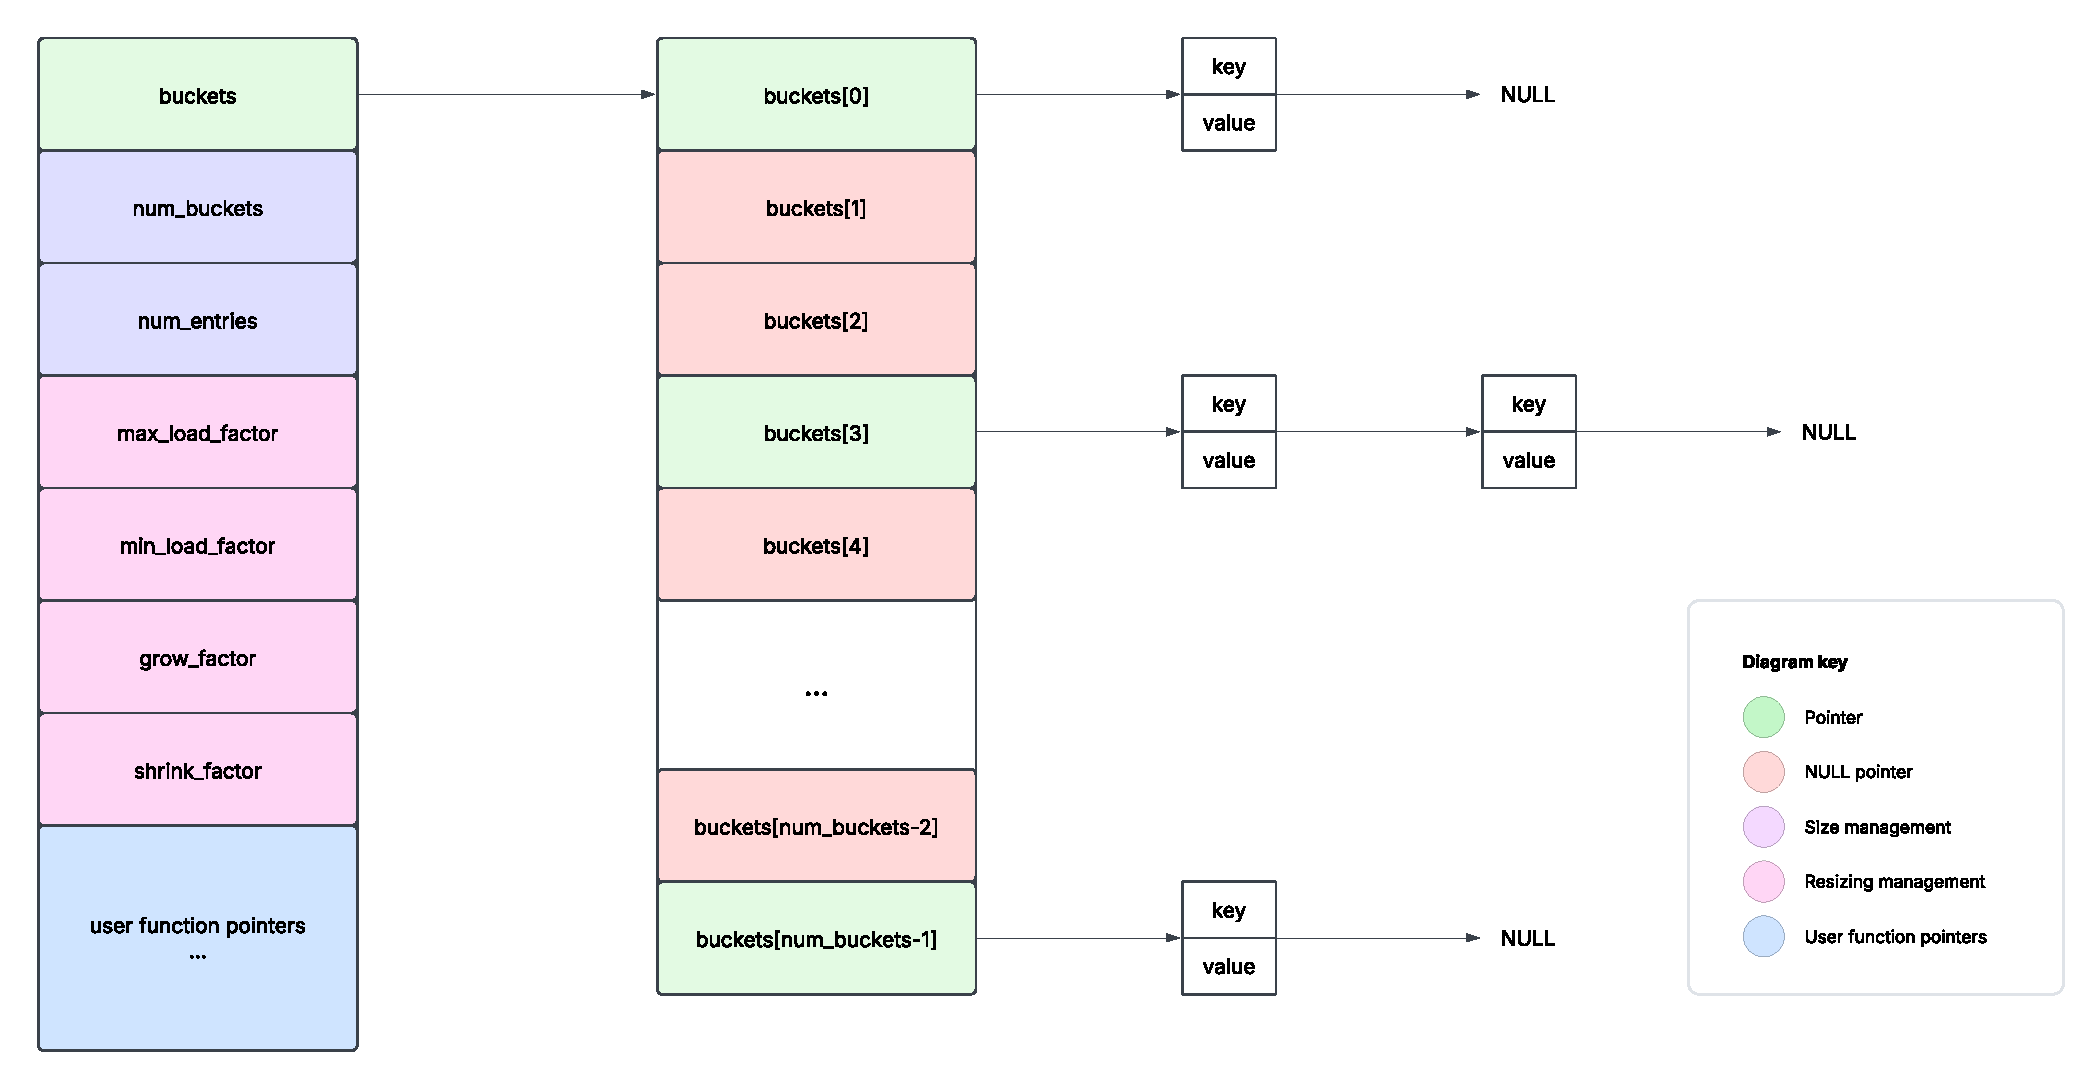
\includegraphics[width=0.8\textwidth]{hashmap_structure.pdf}
    \caption{Hashmap Structure}
    \label{fig:hashmap-structure}
\end{figure}



\subsubsection{Insertion Process}

\textbf{1. Hashing} \\
The hashmap relies on a user-supplied hash function, defined as:
\[
\text{usr\_hash}(\text{key}) \rightarrow \text{unsigned integer}
\]
This function determines the bucket index as follows:
\[
\text{index} = \text{usr\_hash}(\text{key}) \mod \text{num\_buckets}
\]
The efficiency of hashmap operations depends on the quality of this hash function.

\textbf{Example Hash Functions:}
\begin{minted}{c}
// Simple Modulo Hash Function
uint64_t simple_hash(void *key) {
    return (uint64_t)key % 1024;
}

// FNV-1a Hash Function (More Effective)
uint64_t fnv1a_hash(void *key, size_t len) {
    uint64_t hash = 14695981039346656037ULL; // FNV offset basis
    for (size_t i = 0; i < len; i++) {
        hash ^= ((unsigned char*)key)[i];
        hash *= 1099511628211ULL; // FNV prime
    }
    return hash;
}
\end{minted}

\textbf{2. Bucket Selection} \\
Each bucket is an \textbf{entry in an array} indexed using the computed hash value:
\[
\text{buckets[index]}
\]
If \texttt{buckets[index]} is \texttt{NULL}, the bucket is empty, and a new \texttt{map\_element\_t} is allocated. Otherwise, the key-value pair is inserted into the existing linked list at that bucket.


\subsubsection{Collision Handling (Separate Chaining)}

\textbf{Why Do Collisions Happen?} \\
A \textbf{collision} occurs when two different keys hash to the same bucket index. Since the hashmap uses a fixed number of buckets, multiple keys can map to the same index:
\[
\text{index} = \text{usr\_hash}(\text{key}) \mod \text{num\_buckets}
\]
To handle this, the hashmap uses separate chaining, where each bucket points to the head of a linked list storing multiple key-value pairs.
\\
\\

\textbf{How the Hashmap Handles Collisions:} \\
When inserting a new key-value pair:
\begin{itemize}
\item The bucket index is computed using the hash function.
\item If the bucket is empty (\texttt{NULL}), a new element is created and assigned to the bucket.
\item If the bucket already contains elements, the hashmap:
\item Traverses the linked list to check if the key already exists.
\item If the key exists, the value is updated.
\item Otherwise, the new key-value pair is added to the front of the linked list.
\end{itemize}

\textbf{Example: Handling Collisions in Code}
\begin{minted}{c}
map_error_t map_insert(map_t *map, void *key, void *value) {
    if (!map || !key || !value) return MAP_ERR_INVALID_ARG;

    // Compute bucket index
    uint64_t index = map->usr_hash(key) % map->num_buckets;

    // Get the head of the linked list at this bucket
    map_element_t *current = map->buckets[index];

    // Traverse the list to check if the key already exists
    while (current) {
        if (map->usr_compare(current->_key, key) == 0) {
            // Key already exists, update the value
            map->usr_free_value(current->_value);
            current->_value = map->usr_value_clone(value);
            return MAP_OK;
        }
        current = current->_next;
    }

    // If key does not exist, create a new element and insert it at the head
    map_element_t *new_elem = malloc(sizeof(map_element_t));
    if (!new_elem) return MAP_ERR_NO_MEM;

    new_elem->_key = map->usr_key_clone(key);
    new_elem->_value = map->usr_value_clone(value);
    new_elem->_next = map->buckets[index]; // Insert at the front
    map->buckets[index] = new_elem; // Update bucket pointer

    map->num_entries++; // Increment entry count
    return MAP_OK;
}
\end{minted}

\subsubsection{Resizing Strategy}

The hashmap dynamically resizes to ensure efficient performance:

\textbf{1. Growth (Expanding the Number of Buckets)}
\begin{itemize}
    \item When the \textbf{load factor} exceeds $0.75$, the hashmap \textbf{doubles} in size.
    \item A larger bucket array reduces collisions and improves lookup speed.
    \item All elements are rehashed and redistributed across the new bucket array.
\end{itemize}

\textbf{2. Shrinking (Reducing the Number of Buckets)}
\begin{itemize}
    \item When the \textbf{load factor} drops below $0.25$, the hashmap \textbf{shrinks} to half its current size.
    \item This prevents excessive memory usage when fewer elements are stored.
    \item Elements are rehashed into the smaller bucket array.
\end{itemize}

\textbf{3. Why Resizing Matters}
\begin{itemize}
    \item Without resizing, a hashmap can become \textbf{inefficient}, leading to more collisions and slower lookups.
    \item Resizing ensures that lookup time remains \textbf{close to $O(1)$} on average.
\end{itemize}


\begin{figure}[H]
    \centering
    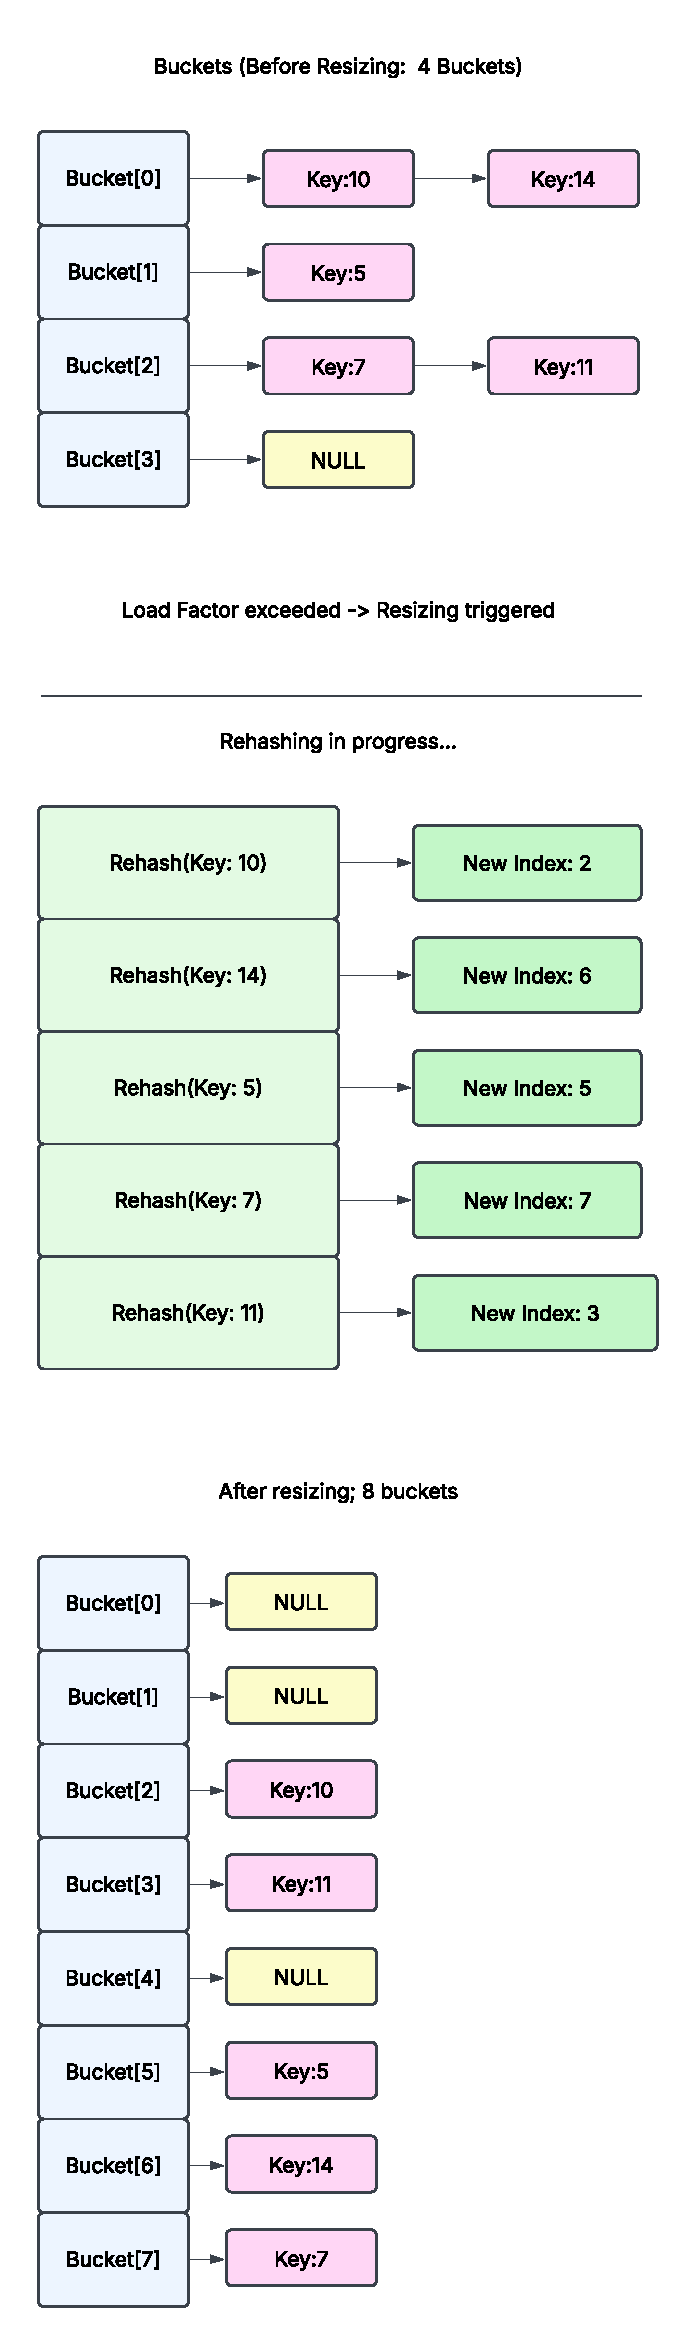
\includegraphics[height=0.8\textheight]{hashmap_resizing.pdf}
    \caption{Resizing process in \texttt{libmap}: Elements are rehashed and moved to new buckets.}
    \label{fig:resizing}
\end{figure}



\subsubsection{Key Takeaways}
\begin{itemize}
    \item \textbf{Buckets are pointers} (\texttt{map\_element\_t **buckets})
    \item \textbf{Each bucket points to a linked list head} (or \texttt{NULL} if empty)
    \item \textbf{Collisions are handled by linked list chaining}
    \item \textbf{Resizing happens dynamically} to maintain efficiency
    \item \textbf{Hashmap grows when load factor $> 0.75$} (to reduce collisions)
    \item \textbf{Hashmap shrinks when load factor $< 0.25$} (to save memory)
    \item \textbf{Good hash functions reduce collisions and improve performance}
\end{itemize}

\subsection{Data Structures}

\subsubsection{\texttt{map\_t} (Hashmap Structure)}
The \texttt{map\_t} structure represents the main hashmap. It stores key-value pairs, handles collisions, and manages resizing.

\textbf{Structure Definition:}
\begin{minted}{c}
typedef struct {
  map_element_t **buckets;  // Array of bucket pointers (linked list heads)
  int32_t num_buckets;      // Current number of buckets
  int32_t num_entries;      // Current number of stored key-value pairs
  float max_load_factor;    // Resizing threshold for growth
  float min_load_factor;    // Resizing threshold for shrinking
  float grow_factor;        // Factor by which the hashmap grows
  float shrink_factor;      // Factor by which the hashmap shrinks

  // User-defined function pointers
  void *(*usr_key_clone)(void *key);
  void *(*usr_value_clone)(void *value);
  uint64_t (*usr_hash)(void *key);
  char *(*usr_stringify)(void *key, void *data);
  int32_t (*usr_compare)(void *key1, void *key2);
  void (*usr_free_key)(void *key);
  void (*usr_free_value)(void *value);
} map_t;
\end{minted}

\textbf{Description:}
This structure contains all necessary information for managing a hashmap, including:
\begin{itemize}
    \item Buckets (\texttt{buckets}) $\rightarrow$ Array of pointers to linked lists for separate chaining.
    \item Load Factors (\texttt{max\_load\_factor}, \texttt{min\_load\_factor}) $\rightarrow$ Control when resizing happens.
    \item Resizing Factors (\texttt{grow\_factor}, \texttt{shrink\_factor}) $\rightarrow$ Determines how much the hashmap expands or shrinks.
    \item User-Defined Functions $\rightarrow$ Custom key-value operations (hashing, comparison, cloning, freeing, stringifying).
\end{itemize}

\textbf{Member Breakdown:}
\begin{center}
\begin{tabular}{@{} l l l @{} }
\toprule
\textbf{Member} & \textbf{Type} & \textbf{Description} \\
\midrule
\texttt{buckets} & \texttt{map\_element\_t**} & Array of bucket pointers (linked list heads) \\
\texttt{num\_buckets} & \texttt{int32\_t} & Number of buckets (size of \texttt{buckets} array) \\
\texttt{num\_entries} & \texttt{int32\_t} & Number of key-value pairs stored \\
\texttt{max\_load\_factor} & \texttt{float} & Threshold for hashmap growth \\
\texttt{min\_load\_factor} & \texttt{float} & Threshold for hashmap shrinking \\
\texttt{grow\_factor} & \texttt{float} & Resizing growth multiplier (e.g., 2.0x) \\
\texttt{shrink\_factor} & \texttt{float} & Resizing shrink multiplier (e.g., 0.5x) \\
\midrule
\multicolumn{3}{l}{\textbf{User-Defined Functions}} \\
\midrule
\texttt{usr\_key\_clone} & \texttt{void *(*)(void*)} & Clones a key (provided by the user) \\
\texttt{usr\_value\_clone} & \texttt{void *(*)(void*)} & Clones a value (provided by the user) \\
\texttt{usr\_hash} & \texttt{uint64\_t (*)(void*)} & Hash function for keys \\
\texttt{usr\_stringify} & \texttt{char *(*)(void*, void*)} & Converts a key-value pair to a string \\
\texttt{usr\_compare} & \texttt{int32\_t (*)(void*, void*)} & Compares two keys \\
\texttt{usr\_free\_key} & \texttt{void (*)(void*)} & Frees a key \\
\texttt{usr\_free\_value} & \texttt{void (*)(void*)} & Frees a value \\
\bottomrule
\end{tabular}
\end{center}

\textbf{Example Usage:}
\begin{minted}{c}
map_t *my_map;
map_create(&my_map, key_clone, value_clone, hash_func,
           stringify_func, compare_func, free_key, free_value);

// Insert some key-value pairs
map_insert(my_map, "name", "Alice");
map_insert(my_map, "age", "25");

// Retrieve a value
char *retrieved_value;
if (map_get(my_map, "name", (void**)&retrieved_value) == MAP_OK) {
    printf("Retrieved: %s\n", retrieved_value);
}

// Cleanup
map_destroy(&my_map);
\end{minted}

\subsubsection{\texttt{map\_element\_t} (Hashmap Node)}
The \texttt{map\_element\_t} structure represents a single key-value pair stored in the hashmap.
Each element is part of a linked list (chaining) used for collision handling.

\textbf{Structure Definition:}
\begin{minted}{c}
typedef struct map_element {
  void *_key;              // Pointer to the key
  void *_value;            // Pointer to the value
  struct map_element *_next; // Pointer to the next element in the bucket
} map_element_t;
\end{minted}

\textbf{Description:}
Each \texttt{map\_element\_t} stores:
\begin{itemize}
    \item A key (\texttt{\_key}) $\rightarrow$ Points to a user-defined key.
    \item A value (\texttt{\_value}) $\rightarrow$ Stores the associated value.
    \item A next pointer (\texttt{\_next}) $\rightarrow$ Links to the next element in the same bucket (if any).
\end{itemize}
Since the hashmap uses separate chaining, multiple elements may exist in a single bucket, forming a linked list.

\textbf{Member Breakdown:}
\begin{center}
\begin{tabular}{@{} l l l @{} }
\toprule
\textbf{Member} & \textbf{Type} & \textbf{Description} \\
\midrule
\texttt{\_key} & \texttt{void*} & Pointer to the stored key \\
\texttt{\_value} & \texttt{void*} & Pointer to the stored value \\
\texttt{\_next} & \texttt{map\_element\_t*} & Pointer to the next element in the bucket (if any) \\
\bottomrule
\end{tabular}
\end{center}


\textbf{Example of a Bucket with Multiple Elements (Collisions)}
\begin{minted}{c}
// Assume 3 keys hash to the same bucket (index 5)
buckets[5] -> [_key="Alice", _value=25] -> [_key="Bob", _value=30] -> NULL
\end{minted}

\textbf{How It Works in the Hashmap:}
- New elements are added at the front of the linked list.
- If a key already exists, its value is updated.
- When an element is removed, the list is properly adjusted.


\begin{figure}[H]
    \centering
    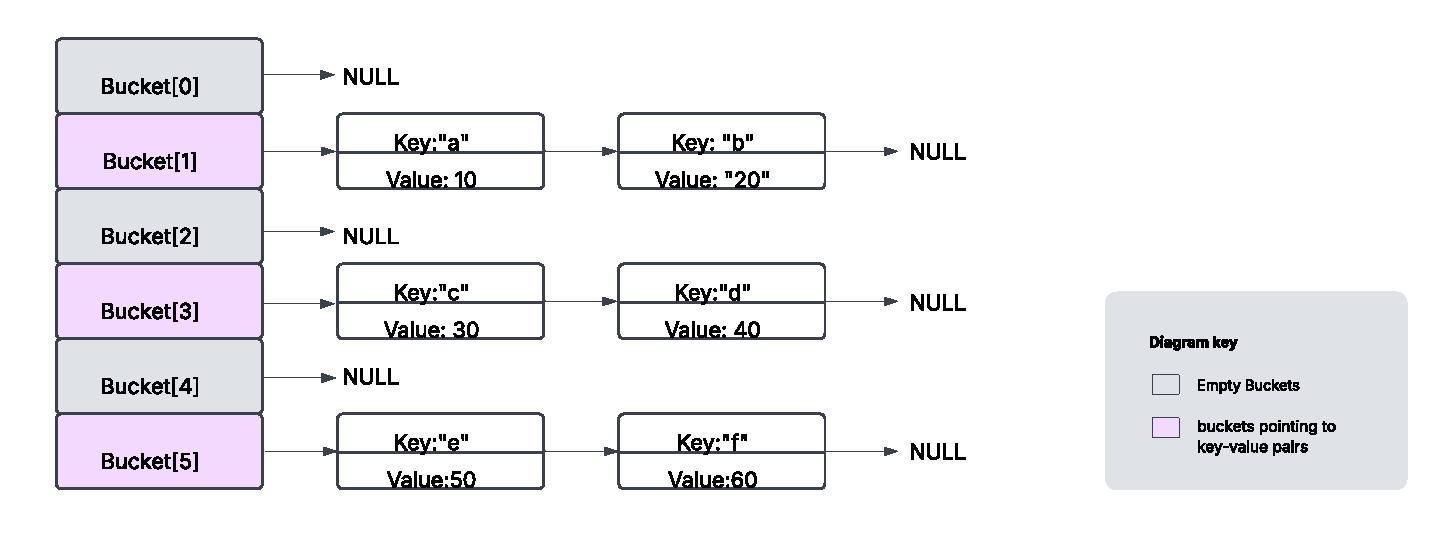
\includegraphics[width=0.8\textwidth]{hashmap_chaining_structure.pdf}
    \caption{Illustration of Bucket Chaining in libmap}
    \label{fig:bucket_chaining}
\end{figure}

\textbf{Example Usage:}
\begin{minted}{c}
map_element_t *elem = malloc(sizeof(map_element_t));
elem->_key = strdup("Alice");
elem->_value = malloc(sizeof(int));
*(int*)elem->_value = 25;
elem->_next = NULL; // First node in the list

// Insert another element in the same bucket
map_element_t *new_elem = malloc(sizeof(map_element_t));
new_elem->_key = strdup("Bob");
new_elem->_value = malloc(sizeof(int));
*(int*)new_elem->_value = 30;
new_elem->_next = elem; // Point to the previous element
elem = new_elem; // Update head of the list
\end{minted}



\subsubsection{\texttt{map\_iterator\_t} (Hashmap Iterator)}
The \texttt{map\_iterator\_t} structure allows users to traverse all elements in the hashmap.

\textbf{Structure Definition:}
\begin{minted}{c}
typedef struct {
  int32_t current_bucket;         // Index of the current bucket
  map_element_t *current_element; // Pointer to the current element in the list
} map_iterator_t;
\end{minted}

\textbf{Description:}
This structure maintains the current position in the hashmap while iterating over elements.

\begin{itemize}
    \item \texttt{current\_bucket} $\rightarrow$ Keeps track of the bucket index in the \texttt{buckets} array.
    \item \texttt{current\_element} $\rightarrow$ Points to the current element in the linked list.
    \item The iterator starts at the first non-empty bucket and moves through the linked lists.
\end{itemize}

\textbf{Iteration Process:}
1. Find the first non-empty bucket and set \texttt{current\_bucket}.
2. Set \texttt{current\_element} to the first key-value pair in that bucket.
3. Move to the next element in the linked list.
4. If the list ends, move to the next non-empty bucket.
5. Repeat until all elements have been visited.

\textbf{Member Breakdown:}
\begin{center}
\begin{tabular}{@{} l l l @{} }
\toprule
\textbf{Member} & \textbf{Type} & \textbf{Description} \\
\midrule
\texttt{current\_bucket} & \texttt{int32\_t} & Index of the current bucket being visited \\
\texttt{current\_element} & \texttt{map\_element\_t*} & Pointer to the current element in the linked list \\
\bottomrule
\end{tabular}
\end{center}

\textbf{Example Usage:}
\begin{minted}{c}
map_iterator_t iter;
map_iter_start(my_map, &iter);

void *key, *value;
while (map_iter_next(my_map, &iter, &key, &value) == MAP_OK) {
    printf("Key: %s, Value: %s\n", (char*)key, (char*)value);
}
\end{minted}

\textbf{How It Works in the Hashmap:}
- \texttt{map\_iter\_start} initializes the iterator at the first valid element.
- \texttt{map\_iter\_next} moves to the next element and retrieves its key-value pair.
- The iteration stops when all elements have been visited.


\subsection{Hashing and Collision Handling}

\subsubsection{What is Hashing?}
A \textbf{hash function} is a function that maps keys to numeric values called \textbf{hash codes}, which determine the bucket index in the hashmap.
\[
\text{index} = \text{usr\_hash}(\text{key}) \mod \text{num\_buckets}
\]
The quality of the hash function significantly impacts hashmap performance.

\begin{figure}[H]
    \centering
    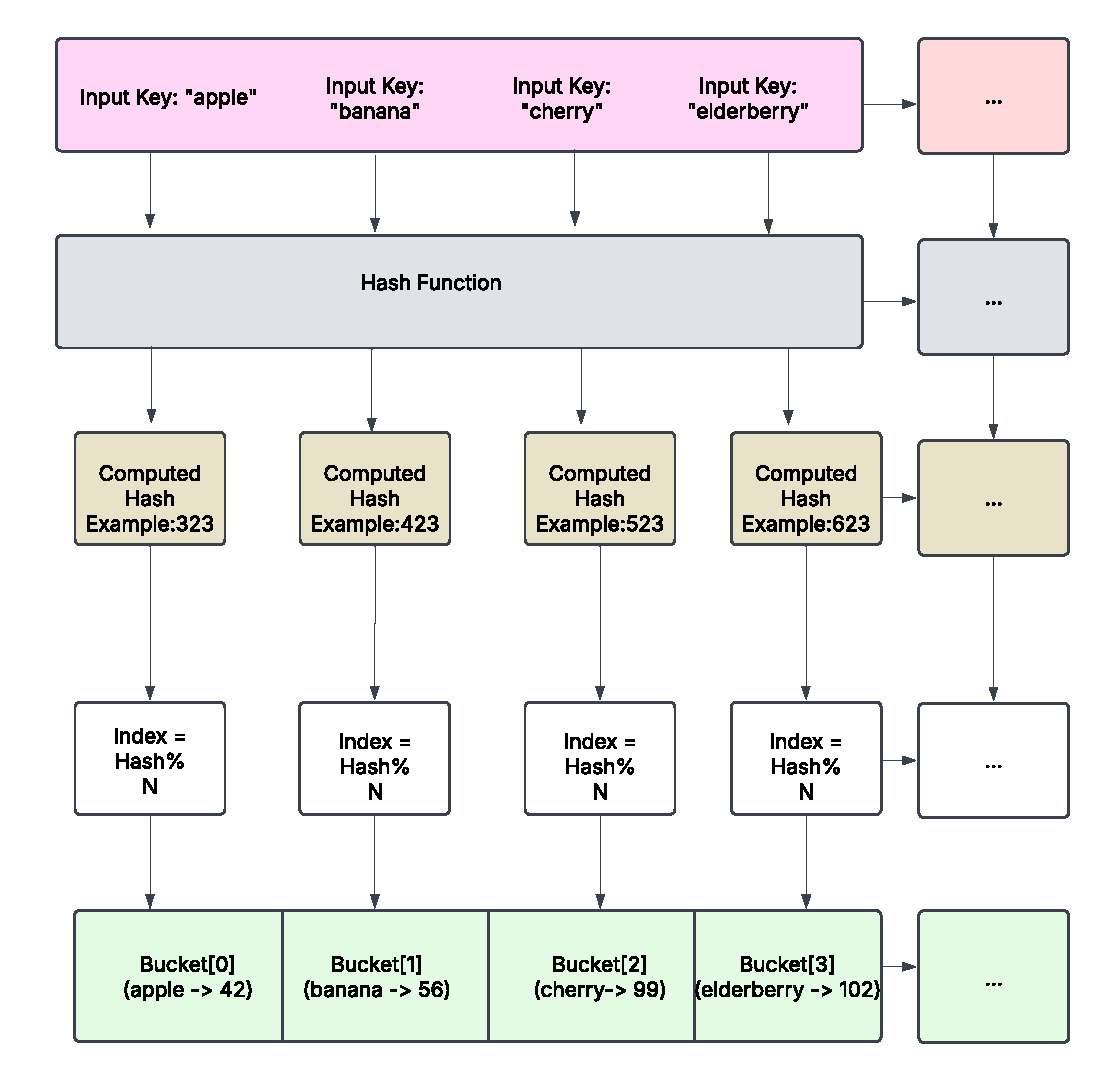
\includegraphics[width=0.8\textwidth]{hash_computation.pdf}
    \caption{Example of Hash Computation and Bucket Indexing}
    \label{fig:hashing}
\end{figure}



\subsubsection{User-Defined Hash Functions}
Unlike some hashmaps that provide built-in hashing, \texttt{libmap} requires the user to define their own hash function via:
\begin{minted}{c}
uint64_t (*usr_hash)(void *key);
\end{minted}
This allows maximum flexibility but requires the user to ensure the function is efficient and well-distributed.

\textbf{Example of a Poor Hash Function (Bad Distribution)}
\begin{minted}{c}
uint64_t bad_hash(void *key) {
    return (uint64_t) key; // Directly returning pointer value (BAD)
}
\end{minted}
This function results in poor distribution, as pointers are not evenly spread across buckets.

\textbf{Example of a Good Hash Function (FNV-1a)}
\begin{minted}{c}
uint64_t fnv1a_hash(void *key, size_t len) {
    uint64_t hash = 14695981039346656037ULL; // FNV offset basis
    for (size_t i = 0; i < len; i++) {
        hash ^= ((unsigned char*)key)[i];
        hash *= 1099511628211ULL; // FNV prime
    }
    return hash;
}
\end{minted}
This function provides strong distribution and reduces clustering.



\subsubsection{Why Do Hash Collisions Happen?}
Since the number of possible keys is much larger than the number of buckets, different keys may hash to the same bucket, causing a \textbf{collision}.
Collisions are unavoidable, so the hashmap must handle them efficiently.

\subsubsection{Collision Handling via Separate Chaining}
\texttt{libmap} resolves collisions using separate chaining, where each bucket contains a linked list of elements.
If multiple keys hash to the same bucket:
1. The first key-value pair is stored in the bucket.
2. The second key-value pair is added as a linked list node.
3. The hashmap traverses the list to retrieve, update, or delete keys.

\textbf{Example: Hash Collision Scenario}
\begin{minted}{c}
// Assume "Alice" and "Bob" hash to the same bucket index (e.g., index 5)
buckets[5] -> [_key="Alice", _value=25] -> [_key="Bob", _value=30] -> NULL
\end{minted}
Inserting "Charlie" at index 5:
\begin{minted}{c}
buckets[5] -> [_key="Charlie", _value=40] -> [_key="Alice", _value=25] -> [_key="Bob", _value=30] -> NULL
\end{minted}
This maintains $O(1)$ insertion in most cases.

\subsubsection{Choosing a Good Hash Function}
A good hash function must:
- Distribute keys uniformly across all buckets.
- Avoid clustering (grouping too many keys in the same bucket).
- Be fast to compute for efficiency.
- Be deterministic (same input always produces the same hash).

\textbf{Comparison of Hash Functions}
\begin{center}
\begin{tabular}{@{} l l l l @{} }
\toprule
\textbf{Hash Function} & \textbf{Speed} & \textbf{Uniformity} & \textbf{Collisions} \\
\midrule
Pointer Casting & Fast & Poor & High \\
Simple Modulo & Fast & Moderate & Moderate \\
FNV-1a & Moderate & Good & Low \\
MurmurHash & Slow & Excellent & Very Low \\
\bottomrule
\end{tabular}
\end{center}

\subsubsection{Alternative Collision Handling Strategies}
\texttt{libmap} uses separate chaining, but other approaches include:
1. Open Addressing -- Instead of linked lists, elements are stored directly in the array, using:
   - Linear Probing $\rightarrow$ Find next available slot.
   - Quadratic Probing $\rightarrow$ Skip slots in increasing steps.
2. Perfect Hashing -- A specialized technique to eliminate collisions but requires extra preprocessing.

\textbf{Why Separate Chaining?}
- Pros: Simple, dynamic resizing is easy, supports variable key sizes.
- Cons: Extra memory for linked lists, can degrade with excessive collisions.

\textbf{Key Takeaways:}
\begin{itemize}
    \item Collisions are inevitable, so they must be handled properly.
    \item \textbf{Separate chaining} is used because it is simple and effective.
    \item A good hash function is crucial for reducing collisions.
    \item Open addressing is another option but is not used in `libmap`.
\end{itemize}

\subsection{Resizing Mechanism}

\subsubsection{Why Resizing is Necessary}
A hashmap must maintain a balance between:
- Efficiency: Ensuring lookups remain fast (\( $O(1)$ \)).
- Memory Usage: Preventing excessive memory allocation.
- Load Factor: Maintaining an optimal bucket-to-element ratio.

Without resizing:
- If the hashmap is too full $\rightarrow$ More collisions occur, degrading performance.
- If the hashmap is too empty $\rightarrow$ Wasted memory, inefficient cache usage.

\subsubsection{When Does Resizing Occur?}
The hashmap automatically resizes when:
\begin{itemize}
    \item Growth Condition: If the number of elements exceeds:
    \[
    \text{max\_load\_factor} \times \text{num\_buckets}
    \]
    The number of buckets increases.
    \item Shrink Condition: If the number of elements falls below:
    \[
    \text{min\_load\_factor} \times \text{num\_buckets}
    \]
    The number of buckets decreases.
\end{itemize}

\textbf{Default Load Factor Values:}
\begin{center}
\begin{tabular}{@{} l l @{} }
\toprule
\textbf{Parameter} & \textbf{Default Value} \\
\midrule
\texttt{max\_load\_factor} & 2.0 (Grow when \texttt{num\_entries} exceeds 2x \texttt{num\_buckets}) \\
\texttt{min\_load\_factor} & 0.5 (Shrink when \texttt{num\_entries} falls below 0.5x \texttt{num\_buckets}) \\
\texttt{grow\_factor} & 2.0 (Buckets double in size) \\
\texttt{shrink\_factor} & 0.5 (Buckets shrink to half) \\
\bottomrule
\end{tabular}
\end{center}

\subsubsection{How Resizing Works (Step-by-Step)}
When resizing is triggered:
1. A new bucket array is allocated with size:
   \[
   \text{new\_num\_buckets} = \text{num\_buckets} \times \text{grow\_factor}
   \]
2. All existing elements are rehashed into the new array.
3. The old bucket array is freed to reclaim memory.

\textbf{Code Implementation of Resizing:}
\begin{minted}{c}
map_error_t __map_resize(map_t *map, float resize_factor) {
    if (!map || resize_factor <= 0) return MAP_ERR_INVALID_ARG;

    uint64_t new_num_buckets = (uint64_t)(map->num_buckets * resize_factor);
    if (new_num_buckets < 1) return MAP_ERR_INVALID_ARG;

    // Allocate new bucket array
    map_element_t **new_buckets = malloc(new_num_buckets * sizeof(map_element_t *));
    if (!new_buckets) return MAP_ERR_NO_MEM;

    // Initialize new buckets
    for (uint64_t i = 0; i < new_num_buckets; i++) new_buckets[i] = NULL;

    // Rehash elements into new bucket array
    for (int i = 0; i < map->num_buckets; i++) {
        map_element_t *current = map->buckets[i];
        while (current) {
            map_element_t *next = current->_next;
            uint64_t new_index = map->usr_hash(current->_key) % new_num_buckets;
            current->_next = new_buckets[new_index];
            new_buckets[new_index] = current;
            current = next;
        }
    }

    // Free old buckets and update hashmap
    free(map->buckets);
    map->buckets = new_buckets;
    map->num_buckets = new_num_buckets;

    return MAP_OK;
}
\end{minted}

\subsubsection{Growth Strategy}
The hashmap grows when:
\[
\text{num\_entries} > \text{max\_load\_factor} \times \text{num\_buckets}
\]
\textbf{Effects of Growing:}
\begin{itemize}
    \item Reduces Collisions $\rightarrow$ More buckets spread out key-value pairs.
    \item Maintains \( $O(1)$ \) Performance $\rightarrow$ Faster lookup times.
    \item Requires Rehashing $\rightarrow$ All elements are redistributed.
\end{itemize}

\textbf{Example: Growth from 4 to 8 Buckets}
\begin{minted}{c}
Before Growth:
buckets[4] -> ["Alice"] -> ["Bob"] -> NULL
buckets[5] -> ["Charlie"] -> NULL

After Growth:
buckets[8] -> ["Alice"] -> NULL
buckets[9] -> ["Bob"] -> NULL
buckets[10] -> ["Charlie"] -> NULL
\end{minted}

\subsubsection{Shrink Strategy}
The hashmap shrinks when:
\[
\text{num\_entries} < \text{min\_load\_factor} \times \text{num\_buckets}
\]
\textbf{Effects of Shrinking:}
\begin{itemize}
    \item Saves Memory $\rightarrow$ Frees unused space.
    \item May Increase Collisions $\rightarrow$ Fewer buckets = more chance of collision.
\end{itemize}

\textbf{Example: Shrinking from 8 to 4 Buckets}
\begin{minted}{c}
Before Shrinking:
buckets[8] -> ["Alice"] -> NULL
buckets[9] -> ["Bob"] -> NULL
buckets[10] -> ["Charlie"] -> NULL

After Shrinking:
buckets[4] -> ["Alice"] -> ["Bob"] -> ["Charlie"] -> NULL
\end{minted}

\subsubsection{Impact of Resizing on Performance}
\textbf{Time Complexity:}
\begin{itemize}
    \item Lookup / Insert / Delete: \( $O(1)$ \) (Amortized)
    \item Resizing (Rehashing): \( $O(n)$ \) (All elements must be moved)
\end{itemize}

\textbf{Trade-offs:}
\begin{itemize}
    \item Pro: Ensures lookup stays efficient.
    \item Pro: Prevents excessive memory use.
    \item Con: Rehashing is expensive (happens rarely).
\end{itemize}

\textbf{Key Takeaways:}
\begin{itemize}
    \item The hashmap grows when it becomes too full (\( > \) max load factor).
    \item The hashmap shrinks when it becomes too empty (\( < \) min load factor).
    \item Resizing helps maintain \( O(1) \) efficiency but has an \( O(n) \) cost.
    \item Choosing a good load factor is essential for performance.
\end{itemize}

\subsection{Iterator Mechanism}

\subsubsection{Why an Iterator is Needed?}
A hashmap stores key-value pairs, but since elements are distributed across multiple buckets (and may have linked lists for collisions), a direct traversal is not possible.
To allow users to efficiently access all elements without exposing internal structures, \texttt{libmap} provides an \textbf{iterator-based API}.

\subsubsection{How Iteration Works}
Iteration involves:
1. Starting at the first non-empty bucket.
2. Retrieving elements from the linked list in that bucket.
3. Moving to the next bucket when the list ends.
4. Repeating until all elements are visited.

\subsubsection{Iterator Structure (\texttt{map\_iterator\_t})}
The iterator tracks the traversal position:
\begin{minted}{c}
typedef struct {
  int32_t current_bucket;         // Index of the current bucket
  map_element_t *current_element; // Pointer to the current element in the list
} map_iterator_t;
\end{minted}

\textbf{Member Breakdown:}
\begin{center}
\begin{tabular}{@{} l l l @{} }
\toprule
\textbf{Member} & \textbf{Type} & \textbf{Description} \\
\midrule
\texttt{current\_bucket} & \texttt{int32\_t} & Index of the bucket currently being iterated \\
\texttt{current\_element} & \texttt{map\_element\_t*} & Pointer to the current element in the linked list \\
\bottomrule
\end{tabular}
\end{center}

\subsubsection{Iterator Functions}
Two functions are provided for iteration:

\textbf{1. Start Iteration (\texttt{map\_iter\_start})}
Initializes the iterator to the first valid key-value pair.

\begin{minted}{c}
map_error_t map_iter_start(const map_t *map, map_iterator_t *iter) {
    if (!map || !iter) return MAP_ERR_INVALID_ARG;

    iter->current_bucket = -1;
    iter->current_element = NULL;

    for (int i = 0; i < map->num_buckets; i++) {
        if (map->buckets[i] != NULL) {
            iter->current_bucket = i;
            iter->current_element = map->buckets[i];
            return MAP_OK;
        }
    }

    return MAP_ERR_END_OF_MAP;
}
\end{minted}

\textbf{2. Retrieve Next Element (\texttt{map\_iter\_next})}
Returns the next key-value pair and advances the iterator.

\begin{minted}{c}
map_error_t map_iter_next(const map_t *map, map_iterator_t *iter,
                          void **out_key, void **out_value) {
    if (!map || !iter || !out_key || !out_value) return MAP_ERR_INVALID_ARG;

    // If inside a bucket's linked list, move to next element
    if (iter->current_element != NULL) {
        *out_key = iter->current_element->_key;
        *out_value = iter->current_element->_value;
        iter->current_element = iter->current_element->_next;
        return MAP_OK;
    }

    // Move to the next non-empty bucket
    while (++iter->current_bucket < map->num_buckets) {
        if (map->buckets[iter->current_bucket] != NULL) {
            iter->current_element = map->buckets[iter->current_bucket];
            *out_key = iter->current_element->_key;
            *out_value = iter->current_element->_value;
            iter->current_element = iter->current_element->_next;
            return MAP_OK;
        }
    }

    return MAP_ERR_END_OF_MAP;
}
\end{minted}

\subsubsection{Example Usage}
\begin{minted}{c}
map_iterator_t iter;
map_iter_start(my_map, &iter);

void *key, *value;
while (map_iter_next(my_map, &iter, &key, &value) == MAP_OK) {
    printf("Key: %s, Value: %s\n", (char*)key, (char*)value);
}
\end{minted}

\subsubsection{Performance Considerations}
\textbf{Time Complexity:}
\begin{itemize}
    \item Best Case: \( $O(1)$ \) per element (if minimal collisions).
    \item Worst Case: \( $O(n)$ \) (if all elements are in a single bucket).
\end{itemize}

\textbf{Trade-offs:}
\begin{itemize}
    \item Pro: Provides a clean way to iterate without exposing internal structure.
    \item Pro: Avoids modifying hashmap state.
    \item Con: Linked list traversal can be slower in high-collision scenarios.
\end{itemize}

\textbf{Key Takeaways:}
\begin{itemize}
    \item The iterator allows users to traverse all elements in a controlled way.
    \item Uses separate chaining, so it must handle linked lists.
    \item Lookup time is \( $O(1)$ \) per element on average, but depends on bucket distribution.
\end{itemize}

\subsection{Trade-offs and Design Choices}

\subsubsection{Choosing Separate Chaining vs. Open Addressing}
A key design choice in \texttt{libmap} was using separate chaining rather than open addressing for collision handling.

\textbf{Why Separate Chaining?}
\begin{itemize}
    \item Handles collisions well -- Each bucket stores a linked list, so multiple keys can exist in the same bucket.
    \item Supports dynamic resizing easily -- Rehashing only requires updating pointers rather than shifting elements.
    \item Works well with variable-sized keys -- Open addressing struggles with non-fixed size data.
    \item Deletion is simple -- Removing an element just involves updating linked list pointers.
\end{itemize}

\textbf{Why Not Open Addressing?}
\begin{itemize}
    \item Suffers from clustering -- Linear/quadratic probing leads to long lookup chains.
    \item More expensive resizing -- Requires rehashing all elements into a new array.
    \item Poor performance at high load factors -- Performance degrades as the table fills up.
\end{itemize}

\textbf{Comparison Table:}
\begin{center}
\begin{tabular}{@{} l l l @{} }
\toprule
\textbf{Technique} & \textbf{Pros} & \textbf{Cons} \\
\midrule
Separate Chaining & Simple, handles collisions well & Uses extra memory for linked lists \\
Open Addressing & Memory efficient & Bad performance with collisions, complex resizing \\
\bottomrule
\end{tabular}
\end{center}

\subsubsection{Dynamic Resizing Strategy}
\texttt{libmap} dynamically resizes when the load factor exceeds a threshold.

\textbf{Why Resize at Load Factor 2.0?}
\begin{itemize}
    \item Keeps collision probability low -- Ensures efficient lookups.
    \item Balances memory usage -- Prevents excessive growth while keeping performance optimal.
\end{itemize}

\textbf{Why Shrink at Load Factor 0.5?}
\begin{itemize}
    \item Avoids wasted space -- Reduces memory footprint when usage decreases.
    \item Prevents excessive allocations/deallocations -- Helps maintain efficiency.
\end{itemize}

\subsubsection{User-Defined Hash Functions: Pros and Cons}
Unlike some libraries that provide built-in hashing, \texttt{libmap} requires the user to define a hash function.

\textbf{Why Allow User-Defined Hash Functions?}
\begin{itemize}
    \item Flexibility -- Users can optimize hash functions for their specific data.
    \item Supports non-standard key types -- Works with custom structs, non-string keys.
    \item Avoids unnecessary computation -- Some applications may already have hashed keys.
\end{itemize}

\textbf{Risks and Potential Issues of User-Defined Functions}
While user-defined functions provide flexibility, they introduce risks that can negatively impact performance and correctness if not implemented carefully.

\textbf{1. Poor Hash Functions Cause Performance Degradation}
\begin{minted}{c}
uint64_t bad_hash(void *key) {
    return 1; // Maps all keys to the same bucket (worst case scenario)
}
\end{minted}

\textbf{2. Hash Functions Must Be Deterministic}
\begin{minted}{c}
uint64_t nondet_hash(void *key) {
    return rand(); // Random values cause lookups to fail
}
\end{minted}

\textbf{3. Comparison Function Errors Can Cause Incorrect Lookups}
\begin{minted}{c}
int bad_compare(void *key1, void *key2) {
    return 2; // Should return 0 for equal keys, nonzero otherwise
}
\end{minted}

\textbf{4. Stringification Functions Can Leak Memory}
\begin{minted}{c}
char *bad_stringify(void *key, void *value) {
    char buffer[100];
    snprintf(buffer, sizeof(buffer), "%s -> %s", (char*)key, (char*)value);
    return buffer; // Returning stack memory! Causes undefined behavior.
}
\end{minted}

\textbf{Best Practices for User-Defined Functions}
To avoid the above issues, follow these rules:
\begin{itemize}
    \item Use strong hash functions like MurmurHash or xxHash.
    \item Ensure the comparison function follows strict equality rules.
    \item Properly free cloned keys and values in deallocation functions.
    \item Test hash distribution by inserting multiple keys and checking for collisions.
\end{itemize}

\subsubsection{Balancing Memory vs. Performance}
Hashmaps must balance speed and memory efficiency.
\texttt{libmap} makes the following design choices:
\begin{itemize}
    \item Optimized for speed -- Keeps lookup, insertion, and deletion at \( $O(1)$ \) time complexity.
    \item Accepts extra memory usage -- Uses linked lists in buckets to handle collisions.
\end{itemize}

\textbf{Memory vs. Performance Trade-offs:}
\begin{center}
\begin{tabular}{@{} l l @{} }
\toprule
\textbf{Optimization} & \textbf{Effect} \\
\midrule
More Buckets & Faster lookups, more memory usage \\
Fewer Buckets & Saves memory, increases collisions \\
Separate Chaining & Easy deletions, more memory overhead \\
Open Addressing & Compact memory, hard to resize \\
\bottomrule
\end{tabular}
\end{center}

\subsubsection{Future Optimizations}
Potential areas for improvement in future versions of \texttt{libmap}:

\textbf{1. Faster Hashing Algorithms}
- Support built-in fast hash functions for common data types.

\textbf{2. Improved Collision Resolution}
- Use linked list sorting to make lookups faster in high-collision scenarios.

\textbf{3. Better Memory Management}
- Reduce malloc/free calls.


\subsubsection{Key Takeaways}
\begin{itemize}
    \item \textbf{Separate Chaining} was chosen over Open Addressing for simplicity and flexibility.
    \item Resizing keeps performance optimal by maintaining a low load factor.
    \item \textbf{User-defined hashing} provides flexibility but requires careful implementation.
    \item Future versions can explore \textbf{built-in fast hash functions, optimized memory management, and smarter iteration}.
\end{itemize}

\newpage

\newpage
% -----------------
% Testing
% -----------------
\section{Testing}

\subsection{Introduction to Testing}

Testing is a \textbf{critical} part of \texttt{libmap}, ensuring that the hashmap implementation behaves correctly under different scenarios. To achieve this, we have designed a \textbf{comprehensive suite of automated tests} that cover various aspects of functionality, correctness, and performance.

All tests in \texttt{libmap} are \textbf{automated}, meaning they run \textbf{without manual intervention}. Each test case uses \textbf{assertions} (\texttt{assert()}) to verify expected behavior, ensuring that any failure \textbf{immediately stops execution} and prints an error message. This approach eliminates the need for manual verification and makes debugging easier.

Additionally, performance testing is a key part of \texttt{libmap} validation. We use \textbf{Flamegraphs} to analyze execution time and identify performance bottlenecks, ensuring that operations like \textbf{insertion, retrieval, and resizing} are efficient even for large datasets.

\subsection{Testing Categories}

Our tests are divided into the following categories:

\begin{itemize}
    \item \textbf{Unit Tests} (Verify individual functions)
    \begin{itemize}
        \item Each function (e.g., \texttt{map\_create()}, \texttt{map\_insert()}, \texttt{map\_get()}) is tested independently.
        \item Tests include \textbf{edge cases}, invalid inputs, and function-specific logic.
    \end{itemize}

    \item \textbf{Integration Tests} (Verify end-to-end correctness)
    \begin{itemize}
        \item Tests real-world scenarios like \textbf{inserting thousands of elements} and ensuring correctness through iteration, retrieval, and removal.
    \end{itemize}

    \item \textbf{Performance Testing with Flamegraphs}
    \begin{itemize}
        \item \texttt{test\_map\_torture.c} runs a \textbf{large-scale performance test} by inserting and manipulating \textbf{10 million key-value pairs}.
        \item A \textbf{Flamegraph} is generated to analyze function execution time and detect slowdowns.
    \end{itemize}

    \item \textbf{Error Handling Tests}
    \begin{itemize}
        \item We simulate failure cases, such as:
        \begin{itemize}
            \item Passing \texttt{NULL} pointers.
            \item Providing broken user-defined functions.
            \item Ensuring correct error codes are returned.
        \end{itemize}
    \end{itemize}
\end{itemize}

By structuring our tests into these categories, \texttt{libmap} ensures \textbf{correctness, robustness, and high performance} under different conditions.

\subsubsection{\texttt{test\_map\_create.c} - Hashmap Creation Test}

\textbf{Purpose:}
This test verifies that the \texttt{map\_create()} function correctly initializes an empty hashmap and properly handles invalid arguments.
It ensures that memory is allocated, internal structures are initialized, and invalid inputs are properly rejected.

\textbf{Test Cases:}
\begin{itemize}
    \item \textbf{Valid Initialization:} Ensures that \texttt{map\_create()} correctly allocates and initializes a hashmap.
    \item \textbf{Invalid Argument Handling:} Tests whether passing \texttt{NULL} as an argument returns an error.
    \item \textbf{Resource Cleanup:} Ensures that the hashmap is correctly deallocated using \texttt{map\_destroy()}.
\end{itemize}

\textbf{Breakdown and Explanation:}
This test covers the following key aspects of \texttt{map\_create()}:

\begin{itemize}
    \item \textbf{Valid Initialization:} The test calls \texttt{map\_create()} with valid function pointers for key cloning, value cloning, hashing, stringifying, comparison, and memory management. If successful, it returns \texttt{MAP\_OK}, confirming that the hashmap has been allocated and initialized properly.
    \item \textbf{Memory Allocation:} The user-defined \texttt{dummy\_int\_key\_clone()} and \texttt{dummy\_int\_value\_clone()} functions allocate memory for cloned keys and values. This ensures that the hashmap owns its copies of inserted data.
    \item \textbf{Hash Function Integration:} The test includes a simple modulus-based hash function \texttt{dummy\_user\_hash()}, which ensures uniform distribution of keys across hashmap buckets.
    \item \textbf{Invalid Argument Handling:} Passing a \texttt{NULL} pointer to \texttt{map\_create()} should return an error (\texttt{MAP\_ERR\_INVALID\_ARG}), preventing segmentation faults or undefined behavior.
    \item \textbf{Cleanup and Destruction:} The test ensures that after the map is created, it is properly cleaned up using \texttt{map\_destroy()}. If \texttt{map\_destroy()} does not correctly free memory, tools like \texttt{valgrind} will report memory leaks.
\end{itemize}

\textbf{Key Validations:}
\begin{itemize}
    \item \texttt{map\_create()} successfully initializes a hashmap.
    \item Passing a \texttt{NULL} pointer returns \texttt{MAP\_ERR\_INVALID\_ARG}.
    \item The allocated hashmap is properly destroyed with \texttt{map\_destroy()}.
\end{itemize}


\subsubsection{\texttt{test\_map\_destroy.c} - Hashmap Destruction Test}

\textbf{Purpose:}
This test ensures that the \texttt{map\_destroy()} function correctly deallocates the hashmap, preventing memory leaks and handling edge cases safely.

\textbf{Test Cases:}
\begin{itemize}
    \item \textbf{Valid Destruction:} Ensures that calling \texttt{map\_destroy()} frees all allocated memory.
    \item \textbf{Repeated Destruction:} Checks if calling \texttt{map\_destroy()} multiple times on the same hashmap is safe.
    \item \textbf{Null Pointer Handling:} Ensures that passing a \texttt{NULL} pointer to \texttt{map\_destroy()} does not cause segmentation faults.
\end{itemize}

\textbf{Breakdown and Explanation:}

This test covers the following key aspects of \texttt{map\_destroy()}:

\begin{itemize}
    \item \textbf{Proper Memory Deallocation:}
    The function should free all allocated memory, including:
    \begin{itemize}
        \item The main \texttt{map\_t} structure.
        \item All stored \texttt{map\_element\_t} nodes.
        \item User-defined keys and values using \texttt{usr\_free\_key()} and \texttt{usr\_free\_value()}.
    \end{itemize}

    \item \textbf{Ensuring Safe Double-Free Protection:}
    - After calling \texttt{map\_destroy()}, the map pointer should be set to \texttt{NULL}.
    - Calling \texttt{map\_destroy()} on an already destroyed hashmap should return \texttt{MAP\_ERR\_INVALID\_ARG} instead of crashing.

    \item \textbf{Handling Edge Cases:}
    - If \texttt{map\_destroy()} is called on an empty map, it should still function correctly.
    - If \texttt{map\_destroy()} is called on a \texttt{NULL} pointer, it should not crash.
\end{itemize}

\textbf{Key Validations:}
\begin{itemize}
    \item \texttt{map\_destroy()} successfully deallocates the hashmap.
    \item Repeated destruction of the same hashmap does not cause errors.
    \item The \texttt{map} pointer is correctly set to \texttt{NULL} after destruction.
\end{itemize}


\subsubsection{\texttt{test\_map\_insert.c} - Hashmap Insertion Test}

\textbf{Purpose:}
This test ensures that the \texttt{map\_insert()} function correctly adds key-value pairs, handles duplicate keys, and triggers resizing when necessary.

\textbf{Test Cases:}
\begin{itemize}
    \item \textbf{Basic Insertion:} Verify that key-value pairs are inserted correctly.
    \item \textbf{Duplicate Key Handling:} Ensure that inserting an existing key updates the associated value.
    \item \textbf{Resizing Behavior:} Test whether the hashmap resizes when the load factor exceeds the threshold.
    \item \textbf{Invalid Arguments:} Ensure that inserting \texttt{NULL} as a key or value is handled properly.
\end{itemize}

\textbf{Breakdown and Explanation:}

This test covers the following key aspects of \texttt{map\_insert()}:

\begin{itemize}
    \item \textbf{Correct Data Insertion:}
    - The test ensures that new key-value pairs are inserted into the hashmap and can be retrieved correctly.

    \item \textbf{Duplicate Key Handling:}
    - When a key that already exists is inserted again, its value should be updated rather than inserting a duplicate entry.

    \item \textbf{Resizing Behavior:}
    - The hashmap dynamically resizes when the number of elements exceeds the configured load factor, preventing excessive collisions.

    \item \textbf{Invalid Argument Handling:}
    - If \texttt{NULL} is passed as a key, \texttt{map\_insert()} should return \texttt{MAP\_ERR\_INVALID\_ARG}.

    \item \textbf{Memory Safety:}
    - Keys and values are cloned before insertion, ensuring that external modifications to original data do not affect stored values.
\end{itemize}

\textbf{Key Validations:}
\begin{itemize}
    \item \texttt{map\_insert()} successfully inserts key-value pairs.
    \item Duplicate keys update existing values instead of creating duplicates.
    \item Hashmap resizes when the threshold is exceeded.
    \item Inserting a \texttt{NULL} key returns \texttt{MAP\_ERR\_INVALID\_ARG}.
    \item The hashmap is properly cleaned up after the test.
\end{itemize}


\subsubsection{\texttt{test\_map\_get.c} - Hashmap Retrieval Test}

\textbf{Purpose:}
This test ensures that the \texttt{map\_get()} function correctly retrieves values associated with keys, properly handles missing keys, and correctly validates the \texttt{usr\_compare} function.

\textbf{Test Cases:}
\begin{itemize}
    \item \textbf{Valid Retrieval:} Ensures that values inserted into the hashmap can be correctly retrieved.
    \item \textbf{Non-Existent Key Handling:} Tests whether retrieving a key that does not exist returns \texttt{MAP\_ERR\_NOT\_FOUND}.
    \item \textbf{Broken Comparison Function:} Checks the behavior when \texttt{usr\_compare} is incorrectly implemented.
\end{itemize}

\textbf{Breakdown and Explanation:}

This test covers the following key aspects of \texttt{map\_get()}:

\begin{itemize}
    \item \textbf{Correct Retrieval:}
    - The test ensures that key-value pairs inserted into the hashmap can be retrieved correctly.

    \item \textbf{Handling of Missing Keys:}
    - If a key is not found, \texttt{map\_get()} should return \texttt{MAP\_ERR\_NOT\_FOUND} instead of an invalid value.

    \item \textbf{Broken Comparison Function Handling:}
    - If the user provides a faulty \texttt{usr\_compare} function that does not return valid comparison values (\{-1, 0, 1\}), the test ensures that \texttt{MAP\_ERR\_UNKNOWN} is returned.

    \item \textbf{Memory Safety:}
    - The function does not modify or free memory that it does not own. The retrieved value is still managed by the hashmap.
\end{itemize}

\textbf{Key Validations:}
\begin{itemize}
    \item \texttt{map\_get()} correctly retrieves values for valid keys.
    \item \texttt{map\_get()} returns \texttt{MAP\_ERR\_NOT\_FOUND} for missing keys.
    \item A faulty \texttt{usr\_compare} function results in \texttt{MAP\_ERR\_UNKNOWN}.
    \item The hashmap remains consistent and free of memory leaks after operations.
\end{itemize}

\subsubsection{\texttt{test\_map\_remove.c} - Hashmap Deletion Test}

\textbf{Purpose:}
This test ensures that the \texttt{map\_remove()} function correctly deletes key-value pairs, properly updates the hashmap size, and handles cases where keys do not exist.

\textbf{Test Cases:}
\begin{itemize}
    \item \textbf{Valid Removal:} Ensures that an existing key-value pair can be removed.
    \item \textbf{Non-Existent Key Handling:} Checks whether attempting to remove a key that does not exist returns \texttt{MAP\_ERR\_NOT\_FOUND}.
    \item \textbf{Hashmap Shrinking:} If many elements are removed, the hashmap should shrink based on the load factor.
\end{itemize}
\textbf{Breakdown and Explanation:}

This test covers the following key aspects of \texttt{map\_remove()}:

\begin{itemize}
    \item \textbf{Correct Deletion:}
    - Ensures that calling \texttt{map\_remove()} correctly deletes a key-value pair.

    \item \textbf{Handling of Missing Keys:}
    - If a key is not found, \texttt{map\_remove()} should return \texttt{MAP\_ERR\_NOT\_FOUND}.

    \item \textbf{Updating Size:}
    - The test verifies that the hashmap size decreases after each successful removal.

    \item \textbf{Shrinking Mechanism:}
    - When many elements are removed, the hashmap should shrink its bucket array if the load factor drops below the configured minimum.

    \item \textbf{Memory Safety:}
    - The function should not modify or free memory that it does not own.
\end{itemize}

\textbf{Key Validations:}
\begin{itemize}
    \item \texttt{map\_remove()} correctly deletes existing keys.
    \item \texttt{map\_remove()} returns \texttt{MAP\_ERR\_NOT\_FOUND} for missing keys.
    \item The hashmap correctly updates its size after removals.
    \item The hashmap correctly shrinks when necessary.
    \item Memory remains consistent and free of leaks.
\end{itemize}


\subsubsection{\texttt{test\_map\_chaining.c} - Collision Handling Test}

\textbf{Purpose:}
This test ensures that the hashmap correctly handles hash collisions using separate chaining.
A custom hash function is used to force all keys into the same bucket, ensuring that chaining is tested.

\textbf{Test Cases:}
\begin{itemize}
    \item \textbf{Forced Collisions:} Ensures multiple keys hash to the same bucket.
    \item \textbf{Retrieval After Collision:} Confirms that all inserted values are retrievable despite collisions.
    \item \textbf{Deletion in Chained Buckets:} Checks that deleting an element from a chained list does not break the structure.
\end{itemize}

\textbf{Breakdown and Explanation:}

This test ensures that separate chaining is working correctly by forcing all keys to hash to the same bucket.

\begin{itemize}
    \item \textbf{Forced Collisions:}
    - A fake hash function returns the same value for all keys, ensuring all elements collide into the same bucket.

    \item \textbf{Insertion and Linked List Growth:}
    - The hashmap must dynamically manage multiple elements in a single bucket as a linked list.

    \item \textbf{Retrieval from a Chained Bucket:}
    - The test confirms that all values can be retrieved even when they are stored in a linked list at the same bucket.

    \item \textbf{Deletion in Chained Buckets:}
    - When an element is removed, the linked list should remain intact, and the remaining elements should still be accessible.

    \item \textbf{Correct Size Updates:}
    - After deletions, \texttt{map\_get\_size()} should reflect the correct number of elements remaining.

    \item \textbf{Memory Safety:}
    - The test ensures that all allocated memory is freed correctly when \texttt{map\_destroy()} is called.
\end{itemize}

\textbf{Key Validations:}
\begin{itemize}
    \item All inserted elements are retrievable, proving chaining works.
    \item After removing an element, the remaining elements in the bucket remain accessible.
    \item The hashmap correctly updates its size after insertions and deletions.
    \item Memory is correctly managed and freed upon destruction.
\end{itemize}


\subsection{Integration Tests}

\textbf{Purpose:}
Integration tests verify that multiple components of the hashmap work together correctly. While unit tests check individual functions in isolation, integration tests ensure that operations like insertion, retrieval, iteration, and removal work as expected in real-world scenarios.

\textbf{Key Focus Areas:}
\begin{itemize}
    \item Ensuring the hashmap maintains consistency when handling a large number of entries.
    \item Validating that insertion, retrieval, and removal operations function correctly when used together.
    \item Testing edge cases like hashmap resizing, iteration over entries, and high-load conditions.
    \item Evaluating the performance of the hashmap under stress (e.g., inserting 10 million elements).
\end{itemize}

The following integration tests have been implemented:
\begin{itemize}
    \item \texttt{test\_map\_consistency.c} -- Inserts and verifies a large number of key-value pairs, removes a range of elements, and checks iteration behavior.
    \item \texttt{test\_mega\_map.c} -- General large-scale test (user-defined behavior).
    \item \texttt{test\_map\_torture.c} -- Inserts 10 million random key-value pairs, modifies them, retrieves values, and then removes all elements.
\end{itemize}

Each test case is designed to ensure that \texttt{libmap} remains reliable, even under extreme workloads.

\subsubsection{\texttt{test\_map\_consistency.c} - Consistency and Iteration Test}

\textbf{Purpose:}
This test verifies the integrity of the hashmap after sequential insertions, retrievals, iterations, and removals.
It ensures:
\begin{itemize}
    \item Elements are stored and retrieved correctly.
    \item The iterator correctly traverses all elements.
    \item Removal correctly reduces the number of elements.
\end{itemize}

\textbf{Test Cases:}
\begin{itemize}
    \item Insert keys in the range $[1, 1000]$, mapping each key to its square.
    \item Verify all inserted keys exist using \texttt{map\_get()}.
    \item Iterate over the map and verify all elements are counted.
    \item Remove elements in the range $[250,750)$.
    \item Iterate again to confirm that exactly 500 elements remain.
\end{itemize}

\textbf{Breakdown and Explanation:}
This test ensures that:
\begin{itemize}
    \item \textbf{Insertion Consistency:} All keys from 1 to 1000 are correctly stored with their square as values.
    \item \textbf{Accurate Retrieval:} Each key is retrieved and checked for correctness.
    \item \textbf{Iterator Validation:} The iterator successfully counts all elements.
    \item \textbf{Correct Removal Behavior:} Keys in the range $[250, 750)$ are removed.
    \item \textbf{Final Consistency Check:} The iterator confirms that 500 elements remain.
\end{itemize}

\subsubsection{\texttt{test\_mega\_map.c} - Large-Scale Hashmap Operations}

\textbf{Purpose:}
This test performs large-scale hashmap operations, including insertion, retrieval, iteration, and removal.
It ensures:
\begin{itemize}
    \item The hashmap can store and manage a variety of string keys.
    \item Retrieval and removal operations work correctly.
    \item The iterator traverses all elements as expected.
    \item The hashmap correctly deallocates memory upon destruction.
\end{itemize}

\textbf{Test Cases:}
\begin{itemize}
    \item Insert multiple key-value pairs into the hashmap.
    \item Retrieve specific elements to verify correctness.
    \item Iterate over the entire hashmap and print all elements.
    \item Remove a key and ensure it is no longer retrievable.
    \item Destroy the hashmap and verify cleanup.
\end{itemize}

\textbf{Breakdown and Explanation:}
This test validates the correctness of:
\begin{itemize}
    \item \textbf{Insertion:} Multiple string keys are inserted into the hashmap.
    \item \textbf{Retrieval:} The function \texttt{map\_get()} correctly retrieves a key-value pair.
    \item \textbf{Iteration:} The iterator traverses and prints all elements.
    \item \textbf{Removal:} The key \texttt{"banana"} is successfully removed.
    \item \textbf{Destruction:} The hashmap is properly deallocated with \texttt{map\_destroy()}.
\end{itemize}

\subsubsection{\texttt{test\_map\_torture.c} - Large-Scale Hashmap Stress Test}

\textbf{Purpose:}
This test evaluates the performance and robustness of the hashmap by inserting, modifying, retrieving, and deleting a large number of elements. It ensures:
\begin{itemize}
    \item The hashmap can handle a large number of entries (10 million).
    \item The insertions and retrievals perform efficiently under high load.
    \item The iteration mechanism functions correctly with large datasets.
    \item The hashmap correctly deallocates memory after bulk removals.
\end{itemize}

\textbf{Test Cases:}
\begin{itemize}
    \item Insert 10 million random key-value pairs.
    \item Iterate over the hashmap and modify all values.
    \item Retrieve random keys and validate modified values.
    \item Remove all elements from the hashmap.
    \item Ensure proper cleanup and memory deallocation.
\end{itemize}
\textbf{Breakdown and Explanation:}
This test ensures the hashmap remains performant and functional under extreme load:
\begin{itemize}
    \item \textbf{Insertion:} 10 million elements are inserted into the hashmap.
    \item \textbf{Iteration and Modification:} The iterator updates all values in the hashmap.
    \item \textbf{Retrieval:} The test verifies the correctness of modified values.
    \item \textbf{Removal:} All elements are deleted, and the hashmap is deallocated.
\end{itemize}

\textbf{Performance Considerations:}
\begin{itemize}
    \item Since the test involves 10 million elements, memory usage should be monitored.
    \item Hash collisions may occur, but the chaining mechanism ensures proper handling.
    \item Using a large prime number (1,000,003) in the hash function improves distribution.
\end{itemize}

\subsection{Summary of Testing}

To ensure the correctness, stability, and efficiency of \texttt{libmap}, we designed a comprehensive test suite covering both \textbf{unit tests} and \textbf{integration tests}. These tests validate that the hashmap behaves as expected across different scenarios, including boundary conditions, error handling, and performance under stress.

\paragraph{What is Testing and Why is it Important?}
In software development, testing is the process of running a program with various inputs to verify its correctness. A well-tested library ensures:
\begin{itemize}
    \item \textbf{Correct behavior}: The library functions work as intended.
    \item \textbf{Reliability}: The library performs consistently under different conditions.
    \item \textbf{Error handling}: The library can detect and gracefully handle invalid inputs.
    \item \textbf{Performance}: The library remains efficient even with large datasets.
    \item \textbf{Memory safety}: No memory leaks or segmentation faults occur.
\end{itemize}

For \texttt{libmap}, we use two main testing strategies: unit testing and integration testing.

\paragraph{Recap of Unit Tests}
Unit tests focus on testing \textbf{one function at a time in isolation}. Each unit test targets a \textbf{specific function} in \texttt{libmap}, ensuring it behaves correctly under normal and edge cases.

\begin{itemize}
    \item \textbf{Correctness}: Ensures functions perform as expected for valid inputs.
    \item \textbf{Error Handling}: Verifies that invalid inputs return appropriate error codes.
    \item \textbf{Memory Management}: Confirms that allocated memory is properly freed to prevent leaks.
\end{itemize}

\textbf{Unit Tests Implemented:}

\begin{table}[h]
    \centering
    \renewcommand{\arraystretch}{1.3}
    \begin{tabular}{@{} l l @{} }
        \toprule
        \textbf{Test Name} & \textbf{Purpose} \\
        \midrule
        \texttt{test\_map\_create.c} & Ensures correct hashmap initialization. \\
        \texttt{test\_map\_destroy.c} & Checks that memory is freed properly. \\
        \texttt{test\_map\_insert.c} & Validates insertion and automatic resizing. \\
        \texttt{test\_map\_get.c} & Ensures key retrieval works and missing keys are handled correctly. \\
        \texttt{test\_map\_remove.c} & Tests removal, ensuring resizing occurs when needed. \\
        \texttt{test\_map\_chaining.c} & Forces hash collisions and verifies separate chaining works correctly. \\
        \bottomrule
    \end{tabular}
    \caption{Overview of Unit Tests in \texttt{libmap}}
\end{table}

\paragraph{Recap of Integration Tests}
Unit tests ensure individual functions work, but integration tests check how multiple functions work together. These tests simulate real-world usage of the hashmap.

\begin{itemize}
    \item \textbf{Consistency}: Ensures that repeated insertions, retrievals, and removals maintain data integrity.
    \item \textbf{Resilience}: Tests whether \texttt{libmap} can handle large datasets and still perform efficiently.
    \item \textbf{Iterator Safety}: Ensures that iterators behave correctly while modifying the hashmap.
\end{itemize}

\textbf{Integration Tests Implemented:}

\begin{table}[h]
    \centering
    \renewcommand{\arraystretch}{1.3}
    \resizebox{\linewidth}{!}{ % Proper scaling
        \begin{tabular}{p{6cm} p{10cm}}
            \toprule
            \textbf{Test Name} & \textbf{Purpose} \\
            \midrule
            \texttt{test\_map\_consistency.c} & Inserts 1000 elements, verifies retrieval, iterates, removes a range, and checks consistency. \\
            \texttt{test\_map\_torture.c} & Inserts ten million elements, modifies values, retrieves keys, and removes all entries. \\
            \texttt{test\_mega\_map.c} & Large-scale tests simulating real-world use cases. \\
            \bottomrule
        \end{tabular}
    }
    \caption{Overview of Integration Tests in \texttt{libmap}}
\end{table}


\paragraph{Key Differences Between Unit and Integration Testing}

\begin{table}[h]
    \centering
    \renewcommand{\arraystretch}{1.3}
    \begin{tabular}{@{} l c c @{} }
        \toprule
        \textbf{Aspect} & \textbf{Unit Testing} & \textbf{Integration Testing} \\
        \midrule
        Scope & Single function & Multiple functions working together \\
        Purpose & Verify function correctness & Ensure system-wide stability \\
        Complexity & Simple, focused tests & More complex interactions \\
        Example & Testing \texttt{map\_insert()} in isolation & Testing insertion, retrieval, and deletion together \\
        \bottomrule
    \end{tabular}
    \caption{Comparison of Unit Testing and Integration Testing}
\end{table}

\paragraph{Why Testing Matters?}
Testing is not just about catching bugs -- it is about guaranteeing that the library is \textbf{reliable, predictable, and performant}. The tests designed for \texttt{libmap} ensure:

\begin{itemize}
    \item \textbf{Correct behavior} under normal and edge-case scenarios.
    \item \textbf{Robust error handling} to prevent crashes and undefined behavior.
    \item \textbf{Memory safety} by ensuring no memory leaks or invalid accesses occur.
    \item \textbf{Performance validation} under high loads.
\end{itemize}

By running these tests across different environments, we increase confidence that \texttt{libmap} can be used in real-world applications without unexpected failures.

\paragraph{Key Takeaways}
\begin{itemize}
    \item \textbf{Unit tests} verify that individual components of \texttt{libmap} function correctly.
    \item \textbf{Integration tests} ensure these components work together seamlessly.
    \item \textbf{Error handling tests} confirm that \texttt{libmap} gracefully handles invalid operations.
\end{itemize}

With a well-structured test profile, we can confidently say that \texttt{libmap} is stable, efficient, and ready for production use.

\subsection{Performance Analysis}

\textbf{Why Analyze Performance?}

Hashmaps are widely used due to their expected $O(1)$ average-case time complexity for insertions, deletions, and lookups. However, real-world performance is influenced by several factors:

\begin{itemize}
    \item \textbf{Collision Resolution:} Excessive collisions can degrade performance to \texttt{O(n)} in worst-case scenarios.
    \item \textbf{Resizing Overhead:} Frequent growth and reallocation of buckets may introduce performance penalties.
    \item \textbf{User-Defined Functions:} Inefficient \texttt{usr\_hash}, \texttt{usr\_compare}, and memory management functions can cause slowdowns.
\end{itemize}

To ensure optimal performance, we conduct runtime profiling to identify bottlenecks and analyze execution time.

\vspace{5mm}

\textbf{Profiling and Runtime Performance}

Profiling helps analyze how much CPU time is spent in different functions, allowing optimization of critical sections. The key profiling metrics include:

\begin{center}
\renewcommand{\arraystretch}{1.3}
\begin{tabular}{@{} l l @{} }
    \toprule
    \textbf{Metric} & \textbf{Description} \\
    \midrule
    Execution Time & Total runtime of hashmap operations. \\
    Function Hotspots & Functions consuming the most CPU time. \\
    Resizing Frequency & Number of hashmap resizes triggered. \\
    Collision Handling Overhead & Time spent resolving key collisions. \\
    \bottomrule
\end{tabular}
\end{center}

\vspace{5mm}

\textbf{Flamegraph Generation for \texttt{test\_map\_torture.c}}

Since \texttt{test\_map\_torture.c} performs over ten million operations, it is the most suitable test for profiling and stress testing. A Flamegraph, which visualizes function execution time, was generated to identify potential inefficiencies.

The next section presents an in-depth analysis of the profiling results from \texttt{test\_map\_torture.c}.

\subsubsection{Performance Analysis: Flamegraph Interpretation}

\textbf{Introduction to Flamegraphs:}
A \textbf{flamegraph} is a visualization of CPU time spent in different functions during execution. The width of each function block represents its proportion of total execution time. Functions lower in the stack are called by the ones above them.

\textbf{Flamegraph for \texttt{test\_map\_torture.c}:}
The performance profile for the large-scale stress test \texttt{test\_map\_torture.c} reveals key computational hotspots, particularly in insertion, resizing, iteration, and removal.

\begin{center}
    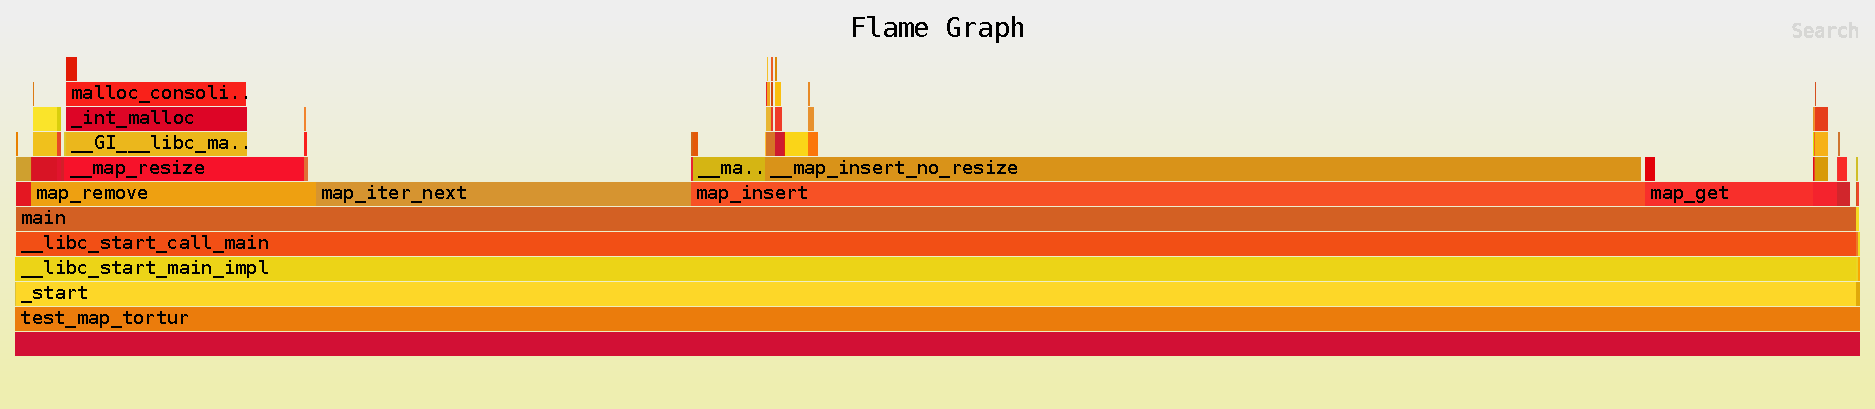
\includegraphics[width=0.9\textwidth]{flamegraph.pdf}
\end{center}

\subsection{Key Performance Insights and Optimization Strategies}

\textbf{Introduction:}
Performance analysis revealed several computational bottlenecks in \texttt{libmap}, primarily during insertion, resizing, iteration, and removal. This section breaks down these challenges, explains why they occur, and proposes optimization strategies to enhance efficiency.

\subsubsection{Identified Bottlenecks}

\begin{itemize}
    \item \textbf{Insertion Costs (\texttt{map\_insert()})}
    Frequent memory allocations for keys, values, and hashmap nodes make insertion expensive, especially when the hashmap grows dynamically.

    \item \textbf{Resizing Overhead (\texttt{\_\_map\_resize()})}
    Resizing involves allocating new buckets, Rehashing all existing keys and moving them to new buckets increases execution time.

    \item \textbf{Iteration Costs (\texttt{map\_iter\_next()})}
    Iterating through a hashmap with chained buckets requires traversing linked lists, which becomes costly when chains grow due to collisions.

    \item \textbf{Deletion Overhead (\texttt{map\_remove()})}
    Removing elements requires searching a bucket and handling chained elements, making it slower when collisions are frequent.

    \item \textbf{Memory Allocation Overhead (\texttt{malloc()})}
    Frequent allocations and deallocations cause fragmentation, impacting overall performance.
\end{itemize}

\subsubsection{Understanding Why These Bottlenecks Occur}

Each of these bottlenecks stems from specific design choices:

\begin{itemize}
    \item \textbf{Insertion Slowness:} Each insertion dynamically allocates memory for keys, values, and nodes, increasing the number of \texttt{malloc()} calls.
    \item \textbf{Resizing Complexity:} When the load factor threshold is exceeded, resizing and rehashing require redistributing all stored elements.
    \item \textbf{Iteration Overhead:} Since elements are stored in linked lists within buckets, iterating requires multiple pointer dereferences.
    \item \textbf{Deletion Cost:} Searching and removing from linked lists involves additional pointer traversals and memory management.
\end{itemize}

\subsubsection{Proposed Optimizations}

The following strategies address the identified bottlenecks:

\begin{table}[h]
    \centering
    \renewcommand{\arraystretch}{1.3}
    \begin{tabular}{@{} l p{6cm} p{4cm} @{}}
        \toprule
        \textbf{Problem} & \textbf{Optimization Strategy} & \textbf{Expected Impact} \\
        \midrule
        Insertion overhead & Use memory pooling to reduce calls to \texttt{malloc()} & Faster insertions, reduced memory fragmentation. \\
        Slow iteration & Optimize bucket traversal (e.g., store precomputed element count) & Faster hashmap iteration. \\
        High deletion costs & Use tombstones instead of immediate deallocation & Faster key removal with deferred memory reuse. \\
        Memory fragmentation & Pre-allocate memory in bulk instead of per-insertion & Reduced allocation overhead and fragmentation. \\
        \bottomrule
    \end{tabular}
    \caption{Optimization Strategies for \texttt{libmap} Performance Improvement}
\end{table}

\subsubsection{Conclusion}

The primary performance constraints in \texttt{libmap} arise from dynamic memory allocation, resizing overhead, and chained traversal during iteration. The proposed optimizations -- reducing unnecessary \texttt{malloc()} calls, improving bucket resizing policies, and refining traversal mechanisms -- can significantly enhance performance.

Further improvements could involve benchmarking different allocation strategies and testing alternate hashing techniques to optimize load distribution.

\subsection{CI/CD using GitHub Actions}

\subsubsection{Introduction to CI/CD}

\textbf{Overview:}  
CI/CD (\textbf{Continuous Integration and Continuous Deployment}) is an automated pipeline that ensures code quality, correctness, and stability. By using \textbf{GitHub Actions}, every commit and push to the repository triggers automated builds and tests, preventing regressions before they reach production.

\textbf{Why CI/CD for \texttt{libmap}?}  
Since \texttt{libmap} is a low-level C library with a strong focus on performance and correctness, CI/CD plays a critical role in ensuring:  
\begin{itemize}  
    \item \textbf{Automated testing:} Every push runs the test suite, catching bugs early.  
    \item \textbf{Memory safety:} Valgrind is used to detect memory leaks and invalid accesses.  
    \item \textbf{Consistent builds:} Ensures that \texttt{libmap} compiles and runs correctly across environments.  
    \item \textbf{Faster debugging:} Immediate feedback from CI logs helps identify and resolve issues quickly.  
\end{itemize}  

\textbf{How GitHub Actions Helps:}  
\texttt{libmap} uses \textbf{GitHub Actions} for CI/CD. This means that \textbf{whenever a developer pushes code}, GitHub automatically:  
\begin{enumerate}  
    \item Checks out the latest code from the repository.  
    \item Installs necessary dependencies (e.g., Valgrind for memory checking).  
    \item Compiles and builds \texttt{libmap}.  
    \item Runs all unit tests and integration tests.  
    \item Runs Valgrind to check for memory leaks.  
    \item Reports results and logs failures if tests fail.  
\end{enumerate}  


\subsubsection{GitHub Actions Workflow}

\textbf{Overview:}  
The CI/CD pipeline for \texttt{libmap} is implemented using a GitHub Actions workflow file. This workflow automates the process of building, testing, and validating the library on every push.  

The workflow file is located at:  
\begin{minted}{text}
.github/workflows/run_hashmap_tests.yml
\end{minted}

\textbf{Workflow Structure:}  
The workflow consists of multiple steps, each performing a key task in the CI/CD pipeline:  

\begin{enumerate}
    \item  The workflow runs on every push to the repository.
    \item  Clones the latest version of the repository.
    \item  Installs necessary tools (e.g., Valgrind).
    \item  Compiles the \texttt{libmap} library.
    \item  Executes all unit and integration tests.
    \item  Runs Valgrind to detect memory leaks.
\end{enumerate}

\textbf{Workflow YAML File:}  
Below is the actual GitHub Actions workflow file used for \texttt{libmap}:  

\begin{minted}{yaml}
name: hashmap regression test

on: [push]

jobs:
  run_hashmap_tests:
    runs-on: ubuntu-latest
    steps:
      - uses: actions/checkout@v3

      - name: Install dependencies
        run: |
          sudo rm /var/lib/man-db/auto-update
          sudo apt-get remove --purge man-db
          sudo apt-get install valgrind

      - name: Build libmap
        run: |
          cd hashmap
          make

      - name: Run all tests
        run: |
          find hashmap/bin -type f -executable | xargs -I {} bash -c '{}; exit $?'

      - name: Valgrind all tests
        run: |
          find hashmap/bin -type f -executable | xargs -I {} bash -c 'valgrind --error-exitcode=1 --leak-check=full --track-origins=yes "{}"; exit $?'
\end{minted}

\textbf{Explanation of Key Steps:}  
\begin{itemize}
    \item \textbf{Checkout Repository:} Retrieves the latest code.
    \item \textbf{Install Dependencies:} Ensures Valgrind is available.
    \item \textbf{Build:} Runs \texttt{make} to compile \texttt{libmap}.
    \item \textbf{Run Tests:} Executes all test cases inside \texttt{hashmap/bin}.
    \item \textbf{Valgrind Analysis:} Runs all tests under Valgrind to detect memory issues.
\end{itemize}

\textbf{Why This Workflow?}  
This workflow ensures that \texttt{libmap} is continuously tested for correctness and memory safety without manual intervention. If any test fails, the workflow provides immediate feedback, allowing developers to fix issues before pushing changes.  



\subsubsection{Interpreting CI Results}

\textbf{Overview:}  
Once the CI/CD workflow is triggered, GitHub Actions provides a detailed log of each step's execution. This section explains how to analyze the results and debug potential failures.

\textbf{Accessing Workflow Logs:}  
To view the CI/CD results:  
\begin{enumerate}
    \item Navigate to the repository on GitHub.
    \item Click on the \textbf{Actions} tab.
    \item Select the most recent workflow run.
    \item Click on individual steps to expand detailed logs.
\end{enumerate}

\textbf{Understanding Test Results:}  
Each step in the workflow outputs a success or failure status. The following table summarizes possible outcomes and their meanings:

\begin{table}[h]
    \centering
    \renewcommand{\arraystretch}{1.3}
    \begin{tabular}{@{} l p{9cm} @{}}
        \toprule
        \textbf{Step} & \textbf{Expected Outcome} \\
        \midrule
        \texttt{Install dependencies} & System dependencies are installed successfully (e.g., Valgrind). \\
        \texttt{Build libmap} & The \texttt{make} command compiles the library without errors. \\
        \texttt{Run all tests} & All unit and integration tests pass with exit code 0. \\
        \texttt{Valgrind all tests} & No memory leaks or invalid accesses detected. \\
        \bottomrule
    \end{tabular}
    \caption{Expected Outcomes for CI/CD Steps}
\end{table}

\textbf{Common Errors and Debugging:}  
If a step fails, the logs provide useful debugging information. Below are common failure scenarios and their solutions:

\begin{table}[h]
    \centering
    \renewcommand{\arraystretch}{1.3}
    \begin{tabular}{@{} l p{9cm} @{}}
        \toprule
        \textbf{Failure} & \textbf{Possible Cause and Fix} \\
        \midrule
        \texttt{Build failed} & Syntax error, missing files, or incorrect \texttt{Makefile}. Check the logs for compilation errors. \\
        \texttt{Tests failed} & A test case failed. Run the tests locally and verify output. \\
        \texttt{Valgrind errors} & Memory leak or invalid access detected. Run tests locally with \texttt{valgrind --leak-check=full}. \\
        \bottomrule
    \end{tabular}
    \caption{Common CI/CD Failures and Debugging Tips}
\end{table}

\textbf{Example: Test Failure Log}  
If a test fails, the logs might show output like this:

\begin{minted}{text}
Running test_map_insert...
Assertion failed...
\end{minted}

This indicates that \texttt{map\_insert()} did not behave as expected. Debugging steps:
\begin{itemize}
    \item Reproduce the failure locally by running \texttt{./bin/test\_map\_insert}.
    \item Use \texttt{printf()} or a debugger to inspect values.
    \item If Valgrind detected a memory issue, analyze the leak report.
\end{itemize}

\textbf{Conclusion:}  
Understanding CI/CD logs is essential for debugging failures efficiently. By analyzing workflow outputs and using local debugging tools, developers can quickly identify and resolve issues.



\subsubsection{Conclusion}

\textbf{CI/CD Ensures Stability:}  
The integration of GitHub Actions into the development workflow of \texttt{libmap} has significantly improved code quality by ensuring that:

\begin{itemize}
    \item Every commit and pull request undergoes rigorous testing.
    \item Memory issues and regressions are detected early using Valgrind.
    \item The build remains stable, preventing broken commits from being merged.
    \item Performance and correctness are continuously validated.
\end{itemize}

\textbf{Key Takeaways:}
\begin{itemize}
    \item Automated Testing: Every push triggers unit and integration tests.
    \item Memory Safety Checks: Valgrind prevents memory leaks.
\end{itemize}


\begin{figure}[H]
    \centering
    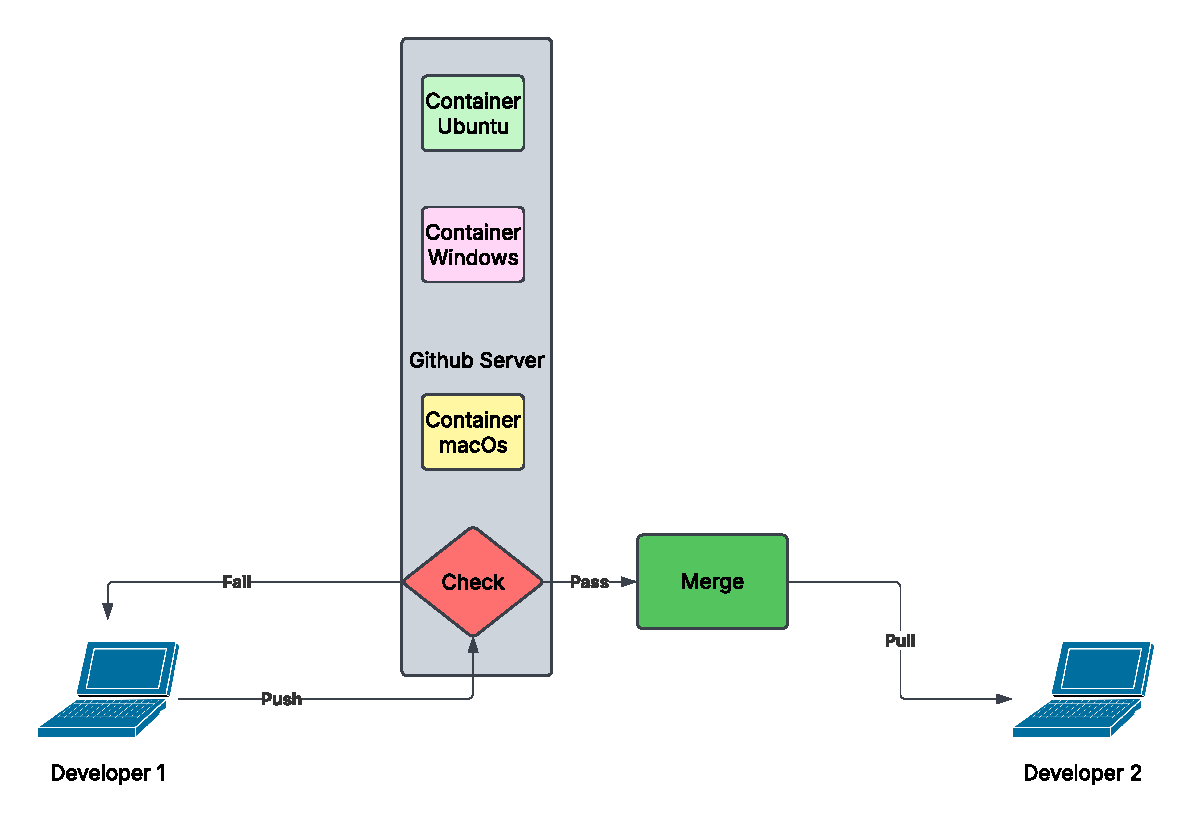
\includegraphics[width=0.9\textwidth]{github_actions.pdf}
    \caption{GitHub Actions Workflow Execution}
    \label{fig:github_actions}
\end{figure}



\textbf{Final Thoughts:}  
CI/CD is a crucial component of modern software development. By leveraging GitHub Actions, \texttt{libmap} ensures stability, reliability, and high performance, allowing developers to focus on feature development rather than manual testing.





\subsection{Final Thoughts on Testing and Performance}

\textbf{Summary of Testing Insights:}
The testing framework for \texttt{libmap} ensures correctness, stability, and efficiency through rigorous unit tests, integration tests, and performance profiling. The unit tests validate individual components such as insertion, retrieval, and removal, while integration tests assess overall consistency and behavior in real-world scenarios. The flamegraph analysis further identifies computational bottlenecks in large-scale operations.

\subsubsection{Strengths of \texttt{libmap}}
The testing and profiling results highlight several strengths of \texttt{libmap}:
\begin{itemize}
    \item \textbf{Efficient Insertion and Retrieval:} The average case complexity for insertion and lookup remains \( $O(1)$ \) with proper hashing.
    \item \textbf{Dynamic Resizing:} Automatic expansion and contraction ensure efficient memory utilization.
    \item \textbf{Customizability:} The library allows user-defined hashing, key comparison, and memory management functions.
    \item \textbf{Iterator Support:} Iterators enable efficient traversal of stored elements.
\end{itemize}

\subsubsection{Identified Weaknesses and Bottlenecks}
Despite its strengths, testing and profiling reveal some areas for improvement:
\begin{itemize}
    \item \textbf{Frequent Resizing Costs:} The flamegraph analysis indicates that reallocation overhead is significant for large datasets.
    \item \textbf{Memory Allocation Overhead:} A considerable portion of execution time is spent in \texttt{malloc()} and \texttt{free()}.
    \item \textbf{Iteration Complexity:} Traversing all elements incurs additional overhead in large hashmaps.
\end{itemize}

\subsubsection{Future Enhancements}
Potential optimizations to enhance performance:
\begin{itemize}
    \item \textbf{Optimized Resizing Strategy:} Switching to power-of-two bucket sizes may reduce resizing overhead.
    \item \textbf{Memory Pooling:} Preallocating memory for elements could reduce dynamic allocation overhead.
    \item \textbf{Improved Collision Resolution:} Exploring alternative techniques like open addressing may improve performance.
\end{itemize}

\textbf{Closing Thoughts:}
The extensive testing and performance profiling of \texttt{libmap} demonstrate its robustness in handling dynamic key-value storage. While the library is efficient for most use cases, optimizations in resizing and memory management can further improve its performance. Future iterations may explore advanced hash functions, alternative data structures, and better memory allocation strategies to enhance overall efficiency.



\subsubsection{Conclusion}

\textbf{CI/CD Ensures Stability:}  
The integration of GitHub Actions into the development workflow of \texttt{libmap} has significantly improved code quality by ensuring that:

\begin{itemize}
    \item Every commit and pull request undergoes rigorous testing.
    \item Memory issues and regressions are detected early using Valgrind.
    \item The build remains stable, preventing broken commits from being merged.
    \item Performance and correctness are continuously validated.
\end{itemize}

\textbf{Key Takeaways:}
\begin{itemize}
    \item Automated Testing: Every push triggers unit and integration tests.
    \item Memory Safety Checks: Valgrind prevents memory leaks.
    \item Optimized Execution: Caching, parallel execution, and logging improve efficiency.
\end{itemize}

\textbf{Final Thoughts:}  
CI/CD is a crucial component of modern software development. By leveraging GitHub Actions, \texttt{libmap} ensures stability, reliability, and high performance, allowing developers to focus on feature development rather than manual testing.



\newpage

% -----------------
% Usage Examples
% -----------------
\section{Usage Examples}
% Detailed examples showing how to use libmap.

\subsection{Counting Unique Elements in an Array}

\textbf{Introduction:}
One of the most common problems in programming is counting the number of unique elements in a dataset.
Traditionally, solutions rely on brute-force checking (\( O(n^2) \)) or sorting followed by a single pass (\( O(n \log n) \)).
However, these methods can be slow, especially for large datasets.

With \texttt{libmap}, we leverage a hashmap-based approach, achieving an optimal $O(n)$ complexity for insertion and lookup.
This makes it significantly faster than sorting, and it scales well for large datasets.

This example demonstrates how \texttt{libmap} makes counting unique elements efficient, readable, and scalable.

\textbf{Implementation:}
\begin{minted}[linenos, breaklines]{c}
#include <stdio.h>
#include <stdlib.h>
#include <assert.h>
#include <string.h>
#include <map.h>

// Dummy key clone function
void* dummy_key_clone(void *key) {
    int *copy = malloc(sizeof(int));
    if (copy) *copy = *(int*)key;
    return copy;
}

// Dummy value clone function
void* dummy_value_clone(void *value) {
    int *new_value = malloc(sizeof(int));
    if (new_value) *new_value = *(int *)value;
    return new_value;
}

// Simple Modulus Hashing
uint64_t dummy_hash(void *key) {
    return (*(int *)key) % 1000003;  // Large prime for better distribution
}

// Dummy stringify function
char* dummy_stringify(void *key, void *value) {
    char *str = malloc(100 * sizeof(char));
    if (str) snprintf(str, 100, "(Key: %d, Value: %d)", *(int *)key, *(int *)value);
    return str;
}

// Dummy compare function
int32_t dummy_compare(void *key1, void *key2) {
    int a = *(int*)key1;
    int b = *(int*)key2;
    return (a > b) - (a < b);
}

// Dummy free functions
void dummy_free_key(void *key) { free(key); }
void dummy_free_value(void *value) { free(value); }

// Function to count unique integers in an array
int count_unique(int *arr, size_t size) {
    map_t *map;
    map_error_t result;

    // Create hashmap
    result = map_create(&map, dummy_key_clone, dummy_value_clone, dummy_hash,
                        dummy_stringify, dummy_compare, dummy_free_key, dummy_free_value);
    assert(result == MAP_OK && "Map creation failed");

    for (size_t i = 0; i < size; i++) {
        int *key = malloc(sizeof(int));
        assert(key && "Memory allocation failed");
        *key = arr[i];

        // Check if the key already exists
        int *existing_freq = NULL;
        result = map_get(map, key, (void **)&existing_freq);

        if (result == MAP_OK) {
            // Key exists, increment its frequency
            (*existing_freq)++;
            free(key);  // Free the unused key
        } else {
            // Key doesn't exist, insert it with frequency = 1
            int *freq = malloc(sizeof(int));
            assert(freq && "Memory allocation failed");
            *freq = 1;

            result = map_insert(map, key, freq);
            assert(result == MAP_OK && "Map insertion failed");
        }
    }

    // Get the number of unique elements
    int unique_count;
    map_get_size(map, &unique_count);

    // Destroy hashmap
    map_destroy(&map);

    return unique_count;
}

// Main function
int main(void) {
    int arr[] = {1,2,2,3,3,4,5,5,6,7,8,8,8,9,10,11,11,11,12};
    size_t size = sizeof(arr) / sizeof(arr[0]); // Convert bytes to elements

    printf("The given array is:\n[");
    for (size_t i = 0; i < size; i++) {
        printf("%d", arr[i]);
        if (i < size - 1) printf(",");
    }
    printf("]\n");

    int unique_count = count_unique(arr, size);
    printf("The number of unique elements in the array is: %d\n", unique_count);

    return 0;
}
\end{minted}

\subsubsection{Breakdown and Explanation}
\begin{itemize}
    \item \textbf{Hashmap-Based Approach:}
        - Instead of iterating multiple times over the array or sorting, we use a hashmap for constant-time lookups.
        - This allows us to count unique elements in linear time $O(n)$.
    \item \textbf{Hashmap Initialization:}
        - The hashmap is created using \texttt{map\_create()} with user-defined functions for key cloning, hashing, comparison, and memory management.
    \item \textbf{Efficient Insertion and Lookup:}
        - Each element is checked in \texttt{map\_get()}.
        - If found, its count is increased.
        - Otherwise, it is inserted into the map.
    \item \textbf{Unique Count Retrieval:}
        - Once all elements are processed, \texttt{map\_get\_size()} returns the number of unique elements.
    \item \textbf{Memory Efficiency:}
        - Since the map dynamically resizes, it scales well with larger datasets.
        - Proper cleanup is ensured with \texttt{map\_destroy()}.
\end{itemize}

\subsubsection{Performance Comparison}
\begin{table}[h]
    \centering
    \renewcommand{\arraystretch}{1.3}
    \begin{tabular}{@{} l l l @{}}
        \toprule
        \textbf{Method} & \textbf{Time Complexity} \\
        \midrule
        Brute Force & \(O(n^2)\)\\
        Sorting + Pass & \(O(n \log n)\) \\
        \texttt{libmap} Hashmap & \($O(n)$\) \\
        \bottomrule
    \end{tabular}
    \caption{Performance Comparison for Counting Unique Elements}
\end{table}

\textbf{Expected Output:}
\begin{minted}{text}
The given array is:
[1,2,2,3,3,4,5,5,6,7,8,8,8,9,10,11,11,11,12]
The number of unique elements in the array is: 10
\end{minted}

\textbf{Key Takeaways:}
\begin{itemize}
    \item Speed: \texttt{libmap} makes the solution fast and scalable with an optimal \texttt{O(n)} complexity.
    \item Readability and Maintainability: Using a hashmap makes the logic clearer and cleaner than manual iteration.
    \item Real-World Impact: This approach can be extended to massive datasets like log analysis, frequency counting, and statistical modeling.
\end{itemize}

\subsection{Other Applications of Hashmaps}

\textbf{Introduction:}
Hashmaps are a fundamental data structure widely used in software development due to their constant-time average complexity for insertions, lookups, and deletions. The \texttt{libmap} library provides a robust, customizable hashmap implementation in C, making it ideal for solving various real-world problems efficiently. Below are some common applications where \texttt{libmap} can be used.

\bigskip

% ------------------------
% Two-Sum Problem
% ------------------------
\textbf{Fast Lookup for the Two-Sum Problem}

\textbf{Use Case:} Given an array of numbers and a target sum, find two numbers that add up to the target.

\textbf{Why Hashmaps?} Instead of a brute-force \(O(n^2)\) approach, a hashmap can store numbers as keys and their indices as values, allowing for quick lookups in \($O(n)$\).

\textbf{How \texttt{libmap} Helps:}
\begin{itemize}
    \item Insert each number into the hashmap with its index as the value.
    \item For each number, check if \texttt{target - num} exists in the hashmap.
    \item If found, return the indices of the two numbers.
\end{itemize}

\bigskip

% ------------------------
% Anagram Checker
% ------------------------
\textbf{Anagram Checker}

\textbf{Use Case:} Determine if two strings are anagrams (contain the same characters in different orders).

\textbf{Why Hashmaps?} Instead of sorting strings (\(O(n \log n)\)), a hashmap can store character frequencies in \($O(n)$\).

\textbf{How \texttt{libmap} Helps:}
\begin{itemize}
    \item Insert characters from the first string into a hashmap as keys, with their counts as values.
    \item Iterate through the second string, decrementing counts.
    \item If all values are zero, the strings are anagrams.
\end{itemize}

\bigskip

% ------------------------
% Key Takeaways
% ------------------------
\textbf{Key Takeaways:}
\begin{itemize}
    \item Hashmaps provide fast lookups and efficient storage for various problems.
    \item \texttt{libmap} enables C programmers to implement these solutions flexibly with custom key-value types.
    \item Using \texttt{libmap}, users can optimize performance-critical applications with frequency counting and efficient data retrieval.
\end{itemize}

\newpage
% -----------------
% Error Handling
% -----------------
\section{Error Handling}
% Explanation of map\_error\_t and error messages.

\subsection{Introduction to Error Handling}
\textbf{Why is error handling important?}
Robust error handling is essential in any library to prevent undefined behavior, crashes, or memory corruption.
\texttt{libmap} is designed with structured error reporting to help users detect and handle failures safely.

\textbf{How does \texttt{libmap} handle errors?}
Unlike some C libraries that rely on \texttt{assert()} or abrupt termination, \texttt{libmap} returns error codes of type \texttt{map\_error\_t}. This allows applications to gracefully handle errors instead of crashing.

\textbf{User responsibility:}
Users of \texttt{libmap} should always check return values from functions and handle errors appropriately. Ignoring errors may lead to undefined behavior or memory leaks.

\textbf{Common failure scenarios:}
\begin{itemize}
    \item \textbf{Invalid arguments:} Passing \texttt{NULL} pointers or incorrect data types.
    \item \textbf{Memory allocation failures:} When \texttt{malloc()} fails due to insufficient memory.
    \item \textbf{Hash collisions:} Large numbers of key collisions could affect performance.
    \item \textbf{Key not found errors:} Attempting to retrieve or remove a key that does not exist.
\end{itemize}

\subsection{\texttt{map\_error\_t}: Error Codes}

\textbf{What is \texttt{map\_error\_t}?}
\texttt{map\_error\_t} is an enumeration that defines error codes returned by \texttt{libmap} functions.
Instead of crashing on errors, functions return meaningful error codes, allowing the user to handle issues safely.

\textbf{Error Code Reference Table:}
The table below summarizes all possible error codes in \texttt{libmap}:

\begin{table}[h]
    \centering
    \renewcommand{\arraystretch}{1.3}
    \begin{tabular}{@{} l p{9cm} @{}}
        \toprule
        \textbf{Error Code} & \textbf{Description} \\
        \midrule
        \texttt{MAP\_OK} & Operation completed successfully. \\
        \texttt{MAP\_ERR\_NO\_MEM} & Memory allocation failed due to insufficient system memory. \\
        \texttt{MAP\_ERR\_NOT\_FOUND} & The requested key was not found in the hashmap. \\
        \texttt{MAP\_ERR\_INVALID\_ARG} & A function received an invalid argument (e.g., NULL pointer). \\
        \texttt{MAP\_ERR\_OVERFLOW} & The hashmap has grown too large to resize further. \\
        \texttt{MAP\_ERR\_END\_OF\_MAP} & Iterator has reached the end of the hashmap. \\
        \texttt{MAP\_ERR\_UNKNOWN} & An unexpected error occurred (should not normally happen). \\
        \bottomrule
    \end{tabular}
    \caption{Error Codes in \texttt{libmap}}
\end{table}

\textbf{When do these errors occur?}
\begin{itemize}
    \item \texttt{MAP\_ERR\_NO\_MEM}: Happens if \texttt{malloc()} fails during allocation.
    \item \texttt{MAP\_ERR\_NOT\_FOUND}: Returned when attempting to retrieve or remove a non-existent key.
    \item \texttt{MAP\_ERR\_INVALID\_ARG}: Occurs when passing a \texttt{NULL} pointer or invalid parameters to a function.
    \item \texttt{MAP\_ERR\_OVERFLOW}: Triggered when the hashmap reaches its maximum allowable size and cannot be resized further.
    \item \texttt{MAP\_ERR\_END\_OF\_MAP}: Used by iterators to signal that no more elements remain in the map.
    \item \texttt{MAP\_ERR\_UNKNOWN}: Indicates an unexpected internal error (should not normally occur).
\end{itemize}

\subsection{How Functions Return Errors}

\textbf{Overview:}
All public functions in \texttt{libmap} return an error code of type \texttt{map\_error\_t}, allowing users to detect and handle issues gracefully.

\subsubsection{Checking Return Values}

To ensure robustness, users should always check the return value of \texttt{libmap} functions before proceeding. Ignoring error codes can lead to undefined behavior, crashes, or memory leaks.

\begin{minted}{c}
map_error_t result = map_insert(my_map, key, value);
if (result != MAP_OK) {
    printf("Error: Failed to insert key (Error Code: %d)\n", result);
}
\end{minted}

\subsubsection{Functions That Return \texttt{map\_error\_t}}

All \texttt{libmap} functions return \texttt{map\_error\_t} to indicate success or failure:

\begin{table}[h]
    \centering
    \renewcommand{\arraystretch}{1.3}
    \begin{tabular}{@{} l l p{6cm} @{}}
        \toprule
        \textbf{Function} & \textbf{Return Type} & \textbf{When to Check Error?} \\
        \midrule
        \texttt{map\_create()} & \texttt{map\_error\_t} & Always check after creation. \\
        \texttt{map\_insert()} & \texttt{map\_error\_t} & Check to ensure insertion succeeded. \\
        \texttt{map\_get()} & \texttt{map\_error\_t} & Handle missing keys properly. \\
        \texttt{map\_remove()} & \texttt{map\_error\_t} & Verify removal success. \\
        \texttt{map\_destroy()} & \texttt{map\_error\_t} & Ensure no double-free occurs. \\
        \bottomrule
    \end{tabular}
    \caption{Error Handling in libmap Functions}
\end{table}

\subsubsection{Best Practices for Error Handling}

\begin{itemize}
    \item \textbf{Always Check Return Values:} Never assume a function succeeded -- always check its return value.
    \item \textbf{Use Meaningful Error Messages:} Instead of just printing \texttt{"Error"}, specify which function failed and why.
    \item \textbf{Handle Critical Errors Immediately:} For issues like \texttt{MAP\_ERR\_NO\_MEM}, consider freeing other resources and aborting gracefully.
    \item \textbf{Log Errors for Debugging:} Use logs to track recurring issues and improve debugging.
\end{itemize}

\subsubsection{Example: Handling Errors Gracefully}

\begin{minted}{c}
map_t *map;
map_error_t result = map_create(&map, key_clone, value_clone, hash, stringify, compare, free_key, free_value);
if (result != MAP_OK) {
    printf("Failed to create hashmap (Error Code: %d)\n", result);
    return 1;
}

char *key = "test";
int value = 42;
result = map_insert(map, key, &value);
if (result != MAP_OK) {
    printf("Failed to insert key: %s (Error Code: %d)\n", key, result);
}
\end{minted}

\subsubsection{Conclusion}

Understanding how \texttt{libmap} functions return errors is crucial for writing stable and reliable code. By checking return values, handling failures properly, and logging errors, users can prevent crashes and ensure smooth hashmap operations.


\subsection{Common Error Scenarios}

\textbf{Overview:}
Errors in \texttt{libmap} typically arise from invalid arguments, memory allocation failures, missing keys, and configuration mistakes. This section covers frequent error cases, their causes, and best practices for handling them.

\subsubsection{Summary of Error Codes}

The following table provides an overview of all error codes defined in \texttt{libmap}:

\begin{table}[h]
    \centering
    \renewcommand{\arraystretch}{1.3}
    \begin{tabular}{@{} l p{8cm} @{}}
        \toprule
        \textbf{Error Code} & \textbf{Description} \\
        \midrule
        \texttt{MAP\_OK} & Operation completed successfully. \\
        \texttt{MAP\_ERR\_NO\_MEM} & Memory allocation failed during an operation. \\
        \texttt{MAP\_ERR\_NOT\_FOUND} & Requested key was not found in the hashmap. \\
        \texttt{MAP\_ERR\_INVALID\_ARG} & One or more arguments passed to a function were invalid. \\
        \texttt{MAP\_ERR\_OVERFLOW} & The table is too large to resize further. \\
        \texttt{MAP\_ERR\_END\_OF\_MAP} & Iterator reached the end of the hashmap. \\
        \texttt{MAP\_ERR\_UNKNOWN} & An unspecified error occurred. \\
        \bottomrule
    \end{tabular}
    \caption{Summary of Error Codes in libmap}
\end{table}


\begin{figure}[H]
    \centering
    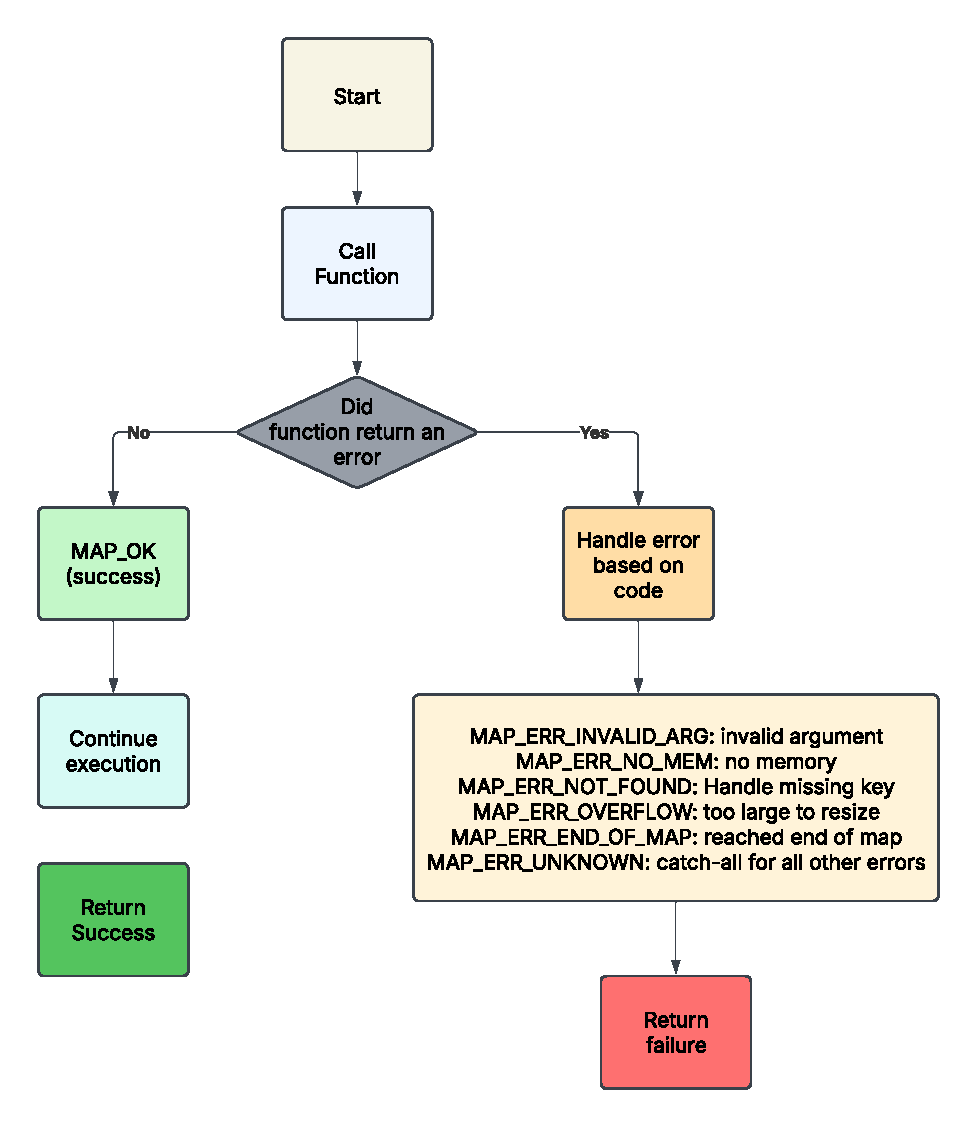
\includegraphics[width=0.75\textwidth]{hashmap_debugging.pdf}
    \caption{Error Handling Flowchart in \texttt{libmap}}
    \label{fig:debugging_flowchart}
\end{figure}



\subsubsection{1. Invalid Arguments (\texttt{MAP\_ERR\_INVALID\_ARG})}

\textbf{Cause:}
Occurs when passing \texttt{NULL} pointers or invalid parameters to a function.

\begin{minted}{c}
// Invalid: Passing NULL as the map pointer
map_error_t result = map_insert(NULL, key, value);
if (result == MAP_ERR_INVALID_ARG) {
    printf("Error: Cannot insert into a NULL map\n");
}
\end{minted}

\textbf{Best Practices:}
\begin{itemize}
    \item Always validate function arguments before calling \texttt{libmap} functions.
    \item Ensure pointers are initialized properly.
    \item Use \texttt{assert()} to catch issues during development.
\end{itemize}

\subsubsection{2. Memory Allocation Failure (\texttt{MAP\_ERR\_NO\_MEM})}

\textbf{Cause:}
Occurs when \texttt{malloc()} fails due to insufficient memory.

\begin{minted}{c}
// Simulating memory failure
void *key = malloc(SIZE_MAX); // Likely to fail
if (key == NULL) {
    printf("Error: Out of memory!\n");
}
\end{minted}

\textbf{Best Practices:}
\begin{itemize}
    \item Always check if \texttt{malloc()} succeeds.
    \item Free memory when no longer needed.
    \item Use tools like Valgrind to detect memory leaks.
\end{itemize}

\subsubsection{3. Key Not Found (\texttt{MAP\_ERR\_NOT\_FOUND})}

\textbf{Cause:}
Occurs when trying to retrieve or remove a key that does not exist.

\begin{minted}{c}
void *value;
map_error_t result = map_get(my_map, "nonexistent", &value);
if (result == MAP_ERR_NOT_FOUND) {
    printf("Error: Key not found in hashmap\n");
}
\end{minted}

\textbf{Best Practices:}
\begin{itemize}
    \item Ensure the key exists before attempting to retrieve it.
    \item Provide meaningful error messages when a key is missing.
    \item Implement fallback behavior for missing keys.
\end{itemize}

\subsubsection{4. Resizing Errors and Configuration Issues (\texttt{MAP\_ERR\_INVALID\_ARG})}

\textbf{Cause:}
Occurs when \texttt{map\_configure()} is called with invalid parameters.

\begin{minted}{c}
// Invalid: grow_factor must be greater than 1
map_error_t result = map_configure(my_map, 100.0, 0.5, 0.9);
if (result == MAP_ERR_INVALID_ARG) {
    printf("Error: Invalid parameters for map configuration\n");
}
\end{minted}

\textbf{Best Practices:}
\begin{itemize}
    \item Set \texttt{max\_load\_factor} and \texttt{min\_load\_factor} carefully.
    \item Ensure \texttt{grow\_factor} is greater than 1.
    \item Validate input parameters before calling \texttt{map\_configure()}.
\end{itemize}

\subsubsection{5. Iterator Errors (\texttt{MAP\_ERR\_END\_OF\_MAP})}

\textbf{Cause:}
Occurs when an iterator reaches the end of the hashmap.

\begin{minted}{c}
map_iterator_t iter;
void *key, *value;
map_error_t result = map_iter_start(my_map, &iter);
while ((result = map_iter_next(my_map, &iter, &key, &value)) == MAP_OK) {
    printf("Key: %s, Value: %d\n", (char *)key, *(int *)value);
}
if (result == MAP_ERR_END_OF_MAP) {
    printf("End of map reached.\n");
}
\end{minted}

\textbf{Best Practices:}
\begin{itemize}
    \item Always check for \texttt{MAP\_ERR\_END\_OF\_MAP} when iterating.
    \item Do not modify the hashmap while iterating.
    \item Reset iterators before reuse.
\end{itemize}

\subsubsection{6. Debugging Tips}

\textbf{Using Assertions for Debugging:}
\begin{minted}{c}
assert(map_insert(my_map, key, value) == MAP_OK);
\end{minted}

\textbf{Using Logging for Error Detection:}
\begin{minted}{c}
map_error_t result = map_insert(my_map, key, value);
if (result != MAP_OK) {
    printf("Error: Failed to insert key. Error code: %d\n", result);
}
\end{minted}

\textbf{Using Valgrind for Memory Errors:}
Run the program with:
\begin{minted}{text}
valgrind --leak-check=full ./test_program
\end{minted}

\subsubsection{Conclusion}

By understanding these common error scenarios and their proper handling, users can ensure robust and predictable behavior when using \texttt{libmap}. Proper error handling minimizes crashes, improves debugging, and enhances application stability.


\subsection{Debugging Tips}

\textbf{Overview:}
Effective debugging of \texttt{libmap} requires both \textbf{preventative measures} (like assertions and compiler warnings) and \textbf{diagnostic tools} (like Valgrind). This section provides techniques to detect and resolve issues efficiently.

\subsubsection{Using Assertions for Error Detection}

Assertions help catch invalid states at runtime. The \texttt{assert()} function from \texttt{<assert.h>} ensures that assumptions hold true during execution.

\begin{minted}{c}
#include <assert.h>

map_t *map = NULL;
assert(map_create(&map, key_clone, value_clone, hash, stringify, compare, free_key, free_value) == MAP_OK);
\end{minted}

\textbf{Use cases:}
\begin{itemize}
    \item Ensuring \texttt{map\_create()} succeeds before proceeding.
    \item Checking if \texttt{map\_get()} successfully retrieves an entry.
    \item Verifying pointer validity before dereferencing.
\end{itemize}

If an assertion fails, the program \textbf{terminates immediately}, helping catch errors early during development.

\subsubsection{Enabling Compiler Warnings}

Compilers provide powerful warnings that help detect potential issues.

\textbf{GCC/Clang Warning Flags:}
\begin{minted}{sh}
gcc -Wall -Wextra -Wpedantic -o test test_map.c -lmap
\end{minted}

\textbf{Use cases:}
\begin{itemize}
    \item Catching \textbf{unused variables, missing return values, and implicit conversions}.
    \item Detecting \textbf{mismatched function signatures} (e.g., passing the wrong argument type).
    \item Preventing \textbf{potential undefined behavior}.
\end{itemize}

Using these flags helps maintain code quality and prevents subtle bugs from slipping into production.

\subsubsection{Using Valgrind for Memory Leak Detection}

Since \texttt{libmap} uses dynamic memory allocation, \textbf{detecting memory leaks} is crucial.

To install Valgrind:
\begin{minted}{sh}
sudo apt install valgrind
\end{minted}

Run it with:
\begin{minted}{sh}
valgrind --leak-check=full --show-leak-kinds=all ./test_map
\end{minted}

\textbf{Use cases:}
\begin{itemize}
    \item Identifying \textbf{memory leaks} in \texttt{map\_create()}, \texttt{map\_insert()}, or \texttt{map\_remove()}.
    \item Checking for \textbf{use-after-free} errors.
    \item Validating that \texttt{map\_destroy()} properly frees memory.
\end{itemize}

\textbf{Example Valgrind output (bad case):}
\begin{minted}{text}
HEAP SUMMARY:
  definitely lost: 32 bytes in 2 blocks
  indirectly lost: 0 bytes in 0 blocks
\end{minted}

If you see "definitely lost" memory, it means some allocated memory was \textbf{not freed}, indicating a potential memory leak.

\subsubsection{Summary of Debugging Techniques}

\begin{table}[h]
    \centering
    \renewcommand{\arraystretch}{1.3}
    \begin{tabular}{@{} l p{10cm} @{}}
        \toprule
        \textbf{Technique} & \textbf{Purpose} \\
        \midrule
        \texttt{assert()} & Catches invalid states during execution. \\
        Compiler Warnings (\texttt{-Wall}, \texttt{-Wextra}) & Detects potential mistakes at compile time. \\
        \textbf{Valgrind} & Identifies memory leaks and use-after-free errors. \\
        \bottomrule
    \end{tabular}
    \caption{Debugging Techniques in libmap}
\end{table}

\subsubsection{Final Thoughts}

\begin{itemize}
    \item \textbf{Use assertions} to detect invalid states early.
    \item \textbf{Enable compiler warnings} to catch issues at compile time.
    \item \textbf{Run Valgrind} to check for memory leaks and improper deallocations.
\end{itemize}

By following these debugging techniques, users can efficiently troubleshoot \texttt{libmap}, prevent crashes, and improve code reliability.


\newpage
% -----------------
% License
% -----------------
\section{License}
% License details.
Copyright 2025 Aditya Singh

Permission is hereby granted, free of charge, to any person obtaining a copy of this software and associated documentation files (the “Software”), to deal in the Software without restriction, including without limitation the rights to use, copy, modify, merge, publish, distribute, sublicense, and/or sell copies of the Software, and to permit persons to whom the Software is furnished to do so, subject to the following conditions:

The above copyright notice and this permission notice shall be included in all copies or substantial portions of the Software.

THE SOFTWARE IS PROVIDED “AS IS”, WITHOUT WARRANTY OF ANY KIND, EXPRESS OR IMPLIED, INCLUDING BUT NOT LIMITED TO THE WARRANTIES OF MERCHANTABILITY, FITNESS FOR A PARTICULAR PURPOSE AND NONINFRINGEMENT. IN NO EVENT SHALL THE AUTHORS OR COPYRIGHT HOLDERS BE LIABLE FOR ANY CLAIM, DAMAGES OR OTHER LIABILITY, WHETHER IN AN ACTION OF CONTRACT, TORT OR OTHERWISE, ARISING FROM, OUT OF OR IN CONNECTION WITH THE SOFTWARE OR THE USE OR OTHER DEALINGS IN THE SOFTWARE.



\newpage
% -----------------
% Contact
% -----------------
\section{Contact}

For any inquiries, feedback, or contributions regarding \texttt{libmap}, feel free to reach out.

\noindent\textbf{Name:} Aditya Singh \\
\noindent\textbf{Email:} \href{mailto:aditherealone@gmail.com}{aditherealone@gmail.com} \\

If you encounter issues or have suggestions for improvements, you are encouraged to report them. Thank you for using \texttt{libmap}!

\end{document}
